\documentclass[conference]{sig-alternate}
%%\documentclass{article} %% hevea
%%\usepackage[utf8]{inputenc} %% hevea

\usepackage[nocompress]{cite}
\usepackage{hyperref}
%% url
\usepackage{url}
%% maths
%%\usepackage[cmex10]{amsmath}
%%\usepackage{amsfonts}
%%\usepackage{amssymb}
%%\usepackage{amsthm}
%% algorithms
\usepackage{algorithm}
\usepackage{algorithmicx}
\usepackage{algpseudocode}
%% images
\usepackage{graphicx}
%% inparaenum
\usepackage[defblank]{paralist}
%% tables
\usepackage{booktabs}
\usepackage{multirow}
%% figures
\usepackage[font=small, skip=5pt]{caption}
\usepackage[font=small]{subfig}
\usepackage{tikz}
\usetikzlibrary{decorations.pathreplacing,plotmarks,shapes,matrix}
%% transform eps in pdf crossplateform
\usepackage{epstopdf}
\usepackage{epsfig}
%% hyphenation
\usepackage{hyphenat}
\hyphenation{brow-sers brow-ser}


\newcommand{\TOFIX}[1]{\textcolor{orange}{#1}}
\newcommand{\TODO}[1]{\textcolor{red}{#1}}

\usepackage{xspace}
\newcommand{\SCAMP}[0]{\textsc{Scamp}\xspace}
\newcommand{\CYCLON}[0]{\textsc{Cyclon}\xspace}
\newcommand{\SPRAY}[0]{\textsc{Spray}\xspace}
\newcommand{\LSEQ}[0]{\textsc{LSeq}\xspace}
\newcommand{\CRATE}[0]{\textsc{Crate}\xspace}
\newcommand{\PEERSIM}[0]{\textsc{PeerSim}\xspace}

\setlength{\belowcaptionskip}{-10pt} %% reduce spacing below figures
\setlength{\intextsep}{7pt} %% reduce spacing on top/bottom of algorithms

\newtheorem{problem}{Problem Statement}
%paralist
\renewcommand*\descriptionlabel[1]{%
\scshape #1}
\renewcommand\paradescriptionlabel[1]{%
\scshape #1}

%%%%%%%%%%%%%%%%%%%%%%%%%%%%%%%%%%%%%%%%%%%%%%%%%%%%%%%%%%%%%%%%%%%%%%%%%%%%%%%
%%%%%%%%%%%%%%%%%%%%%%%%%%%%%%%%%%%%%%%%%%%%%%%%%%%%%%%%%%%%%%%%%%%%%%%%%%%%%%%
%%%%%%%%%%%%%%%%%%%%%%%%%%%%%%%%%%%%%%%%%%%%%%%%%%%%%%%%%%%%%%%%%%%%%%%%%%%%%%%

\begin{document}

\title{An Adaptive Protocol for Building Networks of Browsers}

\numberofauthors{5}
\author{
\alignauthor
Brice N{\'e}delec\\
\affaddr{Universit{\'e} de Nantes, LINA}
%\affaddr{2 rue de la Houssini{\`e}re}\\
%\affaddr{Nantes, FRANCE}\\
\email{brice.nedelec{@}univ-nantes.fr}
\alignauthor
Julian Tanke\\
\affaddr{Universit{\'e} de Nantes, LINA}
%\affaddr{2 rue de la Houssini{\`e}re}\\
%\affaddr{Nantes, FRANCE}\\
\email{julian.tanke{@}fu-berlin.de}
\and
\alignauthor
Davide Frey\\
\affaddr{INRIA Bretagne-Atlantique}
%%\affaddr{Campus Universitaire de Beaulieu}\\
%\affaddr{Rennes, FRANCE}\\
\email{davide.frey@inria.fr}
\alignauthor
Pascal Molli\\
\affaddr{Universit{\'e} de Nantes, LINA}
% \affaddr{2 rue de la Houssini{\`e}re}\\
% \affaddr{Nantes, FRANCE}\\
\email{pascal.molli{@}univ-nantes.fr}
\alignauthor
Achour Mostefaoui\\
\affaddr{Universit{\'e} de Nantes, LINA}
% \affaddr{2 rue de la Houssini{\`e}re}\\
% \affaddr{Nantes, FRANCE}\\
\email{achour.mostefaoui{@}univ-nantes.fr}
}
\date{}

\maketitle

\begin{abstract}
  Deploying peer sampling services on top of WebRTC allows running large scale
  distributed applications on a network of browsers. However, WebRTC has
  several constraints that makes existing peer sampling services inefficient or
  unreliable.  In this paper, we propose \SCAMPLON{}, an adaptive
  peer-sampling service designed to meet the WebRTC constraints. \SCAMPLON{}
  dynamically adapts the neighborhood of each peer to the network
  size. Furthermore, it only uses neighbor-to-neighbor interactions to
  establish the connections and converges exponentially fast to a topology
  exposing similar properties of random graphs. Experiments demonstrate the
  adaptiveness of \SCAMPLON{} and highlight its efficiency improvement compared
  to \CYCLON{} at the cost of a small overhead.
\end{abstract}

%%% Local Variables:
%%% mode: latex
%%% TeX-master: "../paper"
%%% End:



\section{Introduction}

Peer-sampling service is a fundamental mechanism for many large scale
distributed applications including information dissemination,
aggregation or network management~\cite{jelasity2007gossip}. Recently,
WebRTC~\cite{webrtc} opened the opportunity to deploy large scale
distributed application on browsers that can run on laptops, desktops,
tablets or mobile phones. This opportunity is appealing because it
drastically simplify the deployment of large distributed applications
even with complex network settings such as firewall, proxies or Net
Address Translation (NAT).

%Some attractive applications such as Firefox Hello~\cite{firefoxhello}
%or WebTorrent~\cite{webtorrent} demonstrate how video-conferencing or
%file-sharing directly within browsers becomes simple of access to
%end-users without third-party providers.

However, WebRTC has several constraints that makes existing
peer-sampling service inefficient or unreliable. First, browsers can
run on mobile devices and keeping the number of connections as low as
possible is a major requirement. Unfortunately, peer-sampling service
such as \CYCLON{}~\cite{ voulgaris2005cyclon} is not able to adapt the
number of connections to the real number of
participants. Consequently, a user on a mobile phone can maintain 10
connections with others remote browsers, even if just 3 was
enough. Adapting the number of connections to the number of
participants is crucial and is handled by peer-sampling service such
as Scamp~\cite{ganesh2003peer}. Unfortunately, browser-to-browser connection
in WebRTC requires a three-way handshake which is much more costly and
likely to fail compared to traditional settings. We show in this paper
that three-way handshake makes SCAMP fail. 

% PASCAL: too soon, keep that for Pb statement
% Knowingly, the challenge is about
% \begin{inparaenum}[(i)]
% \item keeping an optimal $\Theta(\ln |\mathcal{N}|)$ on the number of
%   connections alive\cite{erdos1959random} (where $\mathcal{N}$ is the set of
%   network members),
% \item keeping an optimal $O(1)$ complexity on connection establishments,
% \item keeping an optimal $\Theta(\exp \, t^{-1})$ convergence speed to a random
%   graph (where $t$ is an arbitrary time frame).
% \end{inparaenum}

In this paper, we introduce \SCAMPLON{}, a random peer sampling
protocol inspired by both \SCAMP{}~\cite{ganesh2003peer} and
\CYCLON{}~\cite{voulgaris2005cyclon}. Compared to state of art,
\begin{inparaenum}[(i)]
\item It dynamically adapts the neighborhood of each peer. Thus, the number of
  connections grows logarithmically compared to the size of the network.
\item It only uses neighbor-to-neighbor interactions to establish the
  connections. Thus, the connections are established in constant time.
\item It converges exponentially fast to a random graph. Thus, the network
  becomes quickly resilient to failure, can broadcast messages
  efficiently etc.
\item In experimental setup, we demonstrate how adaptivity of
  \SCAMPLON{} saves connections compared to\CYCLON{} at the cost of a
  little overhead.
\end{inparaenum}


% Knowingly, it improves state-of-the-art approaches in the traditional
% connection set-up. This improvement is crucial in the three-way connection
% set-up and opens the gate to a vast variety of distributed applications.


The rest of this paper is organized as follow: Section~\ref{sec:background}
introduces the necessary background to understand \SCAMPLON{} and highlights
our motivations. Section~\ref{sec:proposal} details the \SCAMPLON{} protocol.
Section~\ref{sec:experiments} shows the properties of \SCAMPLON{} and compare
them to state-of-the-art random peer sampling
approaches. Section~\ref{sec:relatedwork} reviews the related work. We conclude
and discuss about perspective in Section~\ref{sec:conclusion}.

%%% Local Variables:
%%% mode: latex
%%% TeX-master: "../paper"
%%% End:


\begin{figure*}
\centering
\subfloat[Figure A][\label{fig:webrtcA}
$p_1$ connects to $p_2$ using the signaling service. 
1: $p_1$ pushes its offer ticket; 
2: $p_2$ pulls the ticket; 
3: $p_2$ pushes its response; 
4: $p_1$: pulls the response and establishes a 
connection with $p_2$. $p_3$ does the same with $p_2$. 
%%Figure~\ref{fig:webrtcB} depicts the resulting network.
]{
  
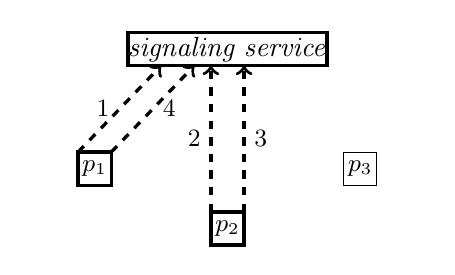
\begin{tikzpicture}[scale=1.2]

\newcommand\X{40pt};
\newcommand\Y{18pt};

\draw( 1.5*\X, 0); %% spacing
\draw(-1.5*\X, 0); %% spacing

\draw[fill=white,very thick](0*\X, 0*\Y) 
node{\emph{signaling service}} +(-30pt,-5pt) rectangle +(30pt,5pt);

\small
\draw[->,dashed, very thick](-5 -1*\X, 5-2*\Y) --
node[anchor=east]{1} (-20pt,-5pt);
\draw[->,dashed, very thick]( 5 -1*\X, 5-2*\Y) --
node[anchor=west]{4} (-10pt,-5pt);

\draw[->,dashed, very thick](-5pt,  5-3*\Y) --
node[anchor=east]{2}(-5pt,-5pt);
\draw[->,dashed, very thick](5pt , 5-3*\Y) --
node[anchor=west]{3} (5pt,-5pt);


\draw[fill=white, very thick]
(-1*\X,-2*\Y) node{$p_1$} +(-5pt,-5pt) rectangle +(5pt,5pt);
\draw[fill=white, very thick]
(0*\X, -3*\Y) node{$p_2$} +(-5pt,-5pt) rectangle +(5pt,5pt);
\draw[fill=white] (1*\X, -2*\Y) node{$p_3$} +(-5pt,-5pt) rectangle +(5pt,5pt);

\end{tikzpicture}

% \begin{tikzpicture}
% \matrix (m) [matrix of math nodes,row sep=4em,column sep=4em] {
% \node(ss)[draw]{signaling}; & \node(p3)[draw]{p3}; \\
% \node(p1)[draw]{p1}; & \node(p2)[draw]{p2}; \\
% };
% \path[->]
%   (p2) edge[dashed] node[fill=white]{1:emit} (ss)
%   (p3) edge[dashed] node[fill=white,bend left]{2:pull} (ss)
%   (p3) edge[dashed, bend right] node[fill=white]{3:accept} (ss)
%   (p2) edge[dashed,bend left] node[fill=white]{4:pull} (ss)
%   (p3) edge[<->,thick] node[fill=white,right]{5:connected} (p2);
% \end{tikzpicture}}
\hspace{5pt}
\subfloat[Figure B][\label{fig:webrtcB}
$p_1$ connects to $p_3$ using $p_2$ as mediator. 
1: $p_1$ sends its offer ticket to $p_2$; 
2: $p_2$ forwards it to $p_3$ and registers $p_1$ as the emitter; 
3: $p_3$ sends its response to $p_2$; 
4: $p_2$ forwards it to the emitter $p_1$ which connects to $p_3$.]{
  
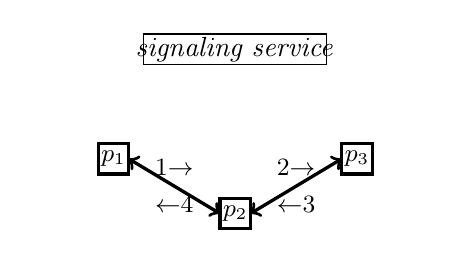
\begin{tikzpicture}[scale=1.1]

\newcommand\X{40pt};
\newcommand\Y{18pt};

\draw(1.7*\X, 0); %% spacing
\draw(-1.7*\X, 0); %% spacing

\draw[fill=white](0*\X, 0*\Y)
node{\emph{signaling service}} +(-30pt,-5pt) rectangle +(30pt,5pt);

\small
\draw[<->, very thick](5-1*\X,-2*\Y)--
node[anchor=south]{1$\rightarrow$}
node[anchor=north]{$\leftarrow$4}(-5pt,-3*\Y);
\draw[<->, very thick](5pt,-3*\Y)--
node[anchor=south]{2$\rightarrow$}
node[anchor=north]{$\leftarrow$3}(-5+1*\X,-2*\Y);

\draw[fill=white, very thick]
(-1*\X,-2*\Y) node{$p_1$} +(-5pt,-5pt) rectangle +(5pt,5pt);
\draw[fill=white, very thick]
(0*\X, -3*\Y) node{$p_2$} +(-5pt,-5pt) rectangle +(5pt,5pt);
\draw[fill=white, very thick]
(1*\X, -2*\Y) node{$p_3$} +(-5pt,-5pt) rectangle +(5pt,5pt);

\end{tikzpicture}

% \begin{tikzpicture}
% \matrix (m) [matrix of math nodes,row sep=4em,column sep=4em] {
% \node(ss)[draw]{signaling}; & \node(p3)[draw]{p3}; \\
% \node(p1)[draw]{p1}; & \node(p2)[draw]{p2}; \\
% };
% \path[->]
%   (p1) edge[dashed,bend left] node[fill=white]{1:emit} (p2)
%   (p2) edge[dashed,bend left] node[fill=white,left]{2:emit/p1} (p3)
%   (p3) edge[dashed,bend left] node[fill=white,right]{3:accept/p1} (p2)
%   (p2) edge[dashed,bend left] node[fill=white]{4:accept} (p1)
%   (p1) edge[<->,thick] (p2)
% %  (p1) edge[<->,thick,bend left] (p3)
%   (p2) edge[<->,thick]  (p3);

% \end{tikzpicture}}
\hspace{5pt}
\subfloat[Figure C][\label{fig:webrtcC}
The resulting network overlay: a fully connected network composed of
3 members.]{
  
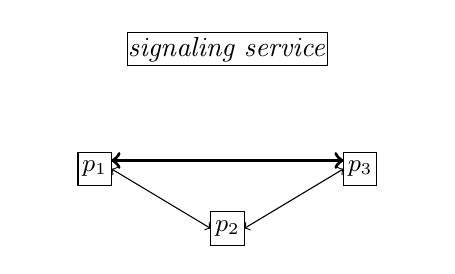
\begin{tikzpicture}[scale=1.2]

\newcommand\X{40pt};
\newcommand\Y{18pt};

\draw(1.5*\X, 0); %% spacing
\draw(-1.5*\X, 0); %% spacing

\draw[fill=white](0*\X, 0*\Y)
node{\emph{signaling service}} +(-30pt,-5pt) rectangle +(30pt,5pt);

\small
\draw[<->](5-1*\X,-2*\Y)--(-5pt,-3*\Y);
\draw[<->](5pt,-3*\Y)--(-5+1*\X,-2*\Y);
\draw[<->, very thick](5 - 1*\X, 2.5 -2*\Y)--(-5+1*\X, 2.5 -2*\Y);

\draw[fill=white]
(-1*\X,-2*\Y) node{$p_1$} +(-5pt,-5pt) rectangle +(5pt,5pt);
\draw[fill=white]
(0*\X, -3*\Y) node{$p_2$} +(-5pt,-5pt) rectangle +(5pt,5pt);
\draw[fill=white]
(1*\X, -2*\Y) node{$p_3$} +(-5pt,-5pt) rectangle +(5pt,5pt);

\end{tikzpicture}


% \begin{tikzpicture}
% \matrix (m) [matrix of math nodes,row sep=4em,column sep=4em] {
% \node(ss)[draw]{signaling}; & \node(p3)[draw]{p3}; \\
% \node(p1)[draw]{p1}; & \node(p2)[draw]{p2}; \\
% };
% \path[->]
%   (p1) edge[<->,thick] (p2)
%   (p1) edge[<->,thick] (p3)
%   (p2) edge[<->,thick]  (p3);
% \end{tikzpicture}}
\caption{\label{fig:webrtc}Creating an overlay network on top of WebRTC.}
\end{figure*}


\section{Related work}
\label{sec:relatedwork}


WebRTC allows real-time peer-to-peer communication between browsers even when
complex network settings such as firewalls, proxies or Net Address Translation
(NAT) are involved. However, WebRTC does not manage addressing nor routing. To
establish a connection, the browsers exchange offers and acknowledgments through
a common mediator, e.g., mails, dedicated signaling services~\cite{peerjs},
existing WebRTC connections~\cite{p} etc. Figure~\ref{fig:webrtcA} describes the
very first connection of one peer $p_1$ with another
$p_2$. Figure~\ref{fig:webrtcB} shows that $p_3$ is able to use $p_2$ as
mediator instead of the signaling service. Figure~\ref{fig:webrtcC} shows the
resulting network. Notice that if $p_2$ crashes during the forwarding process,
the connection establishment will fail, even if an alternative route exists as
WebRTC does not manage routing.

% In Figure~\ref{fig:webrtcA}, $p_1$
% wants to connect to $p_2$. Therefore, $p_1$ pushes an offer ticket to a shared
% signaling service. It is worth noting that many signaling services can
% exist. Peer $p_2$ pulls the offer, stamps it and pushes it back to the signaling
% service. Finally, $p_1$ pulls the stamped ticket and establishes a bidirectional
% connection with $p_2$.  Identically, $p_3$ establishes a connection to $p_2$. We
% refer to the round-trip procedure as \emph{three-way handshake}. At this point,
% Peer $p_1$ is able to establish a connection to $p_3$ without the mediation of
% the former signaling service.  Instead, it uses $p_2$ as temporary signaling
% service.  As shown in Figure~\ref{fig:webrtcB}, Peer $p_1$ pushes an offer
% ticket to $p_2$. As $p_2$ is already connected to $p_3$, it forwards the offer
% to $p_3$ and registers $p_1$ as the emitter. Peer $p_3$ stamps the ticket and
% sends it back to $p_2$ who then forwards it back to $p_1$. Upon receipt, $p_1$
% establishes a bidirectional connection with $p_3$.  Notice that if $p_2$ crashes
% during the forwarding process, the connection establishment will fail, even if
% an alternative route exists as WebRTC does not manage routing.

Using signaling services and existing WebRTC connections allows easy
deployment of random peer sampling protocols~\cite{jelasity2004peer} in
browsers that can run on mobile phones or tablets connected to mobile
networks. In this context, it is crucial to keep the number of connections as
low as possible in order to reduce traffic usage and limit resource
consumption.

Random peer sampling protocols~\cite{jelasity2004peer, jelasity2007gossip}
provide each peer with a partial view $\mathcal{P}$ of the network membership
$\mathcal{N}$. They populate the partial views with references to peers chosen
at random among $\mathcal{N}$ following a uniform distribution using local
knowledge only. Their goal is to converge to an overlay network exposing
properties similar to those of random graphs~\cite{erdos1959random}. They
efficiently provide connectedness, robustness, information dissemination etc. A
wide variety of gossip-based protocols use random peer sampling at their
core. For instance, topology optimization protocols~\cite{voulgaris2005epidemic,
  jelasity2009tman} aim to improve criteria such as localization, latency,
preferences etc.

The representatives of random peer sampling protocols using a fixed-size partial
view are Lpbcast~\cite{eugster2003lightweight},
HyParView\cite{leitao2007hyparview} Newscast~\cite{tolgyeski2009adaptive}, and
\CYCLON~\cite{voulgaris2005cyclon}. They have to know \emph{a priori} the
maximum network size to set their parameters accordingly. These decisions cannot
be safely retracted afterwards.

This inflexibility makes it possible to maintains 7 connections in the browser
despite requiring only 4, while, in the following moment, it still maintains 7
connections while 10 would be needed.  \CYCLON's partial views are commonly
oversized compared to the actual network size to prevent having too few
connections per peer, which, consequently, introduces overhead.  When WebRTC is
involved, we need a dynamic peer sampling service that is able to adapt to the
dynamic number of participants.

Network size estimators can introduce adaptiveness in peer sampling. These
approaches either use
\begin{inparaenum}[(i)]
\item sampling techniques~\cite{ganesh2007peer} which analyze a network subset
  and deduce the network size using probabilistic functions,
\item sketching techniques~\cite{baquero2012extrema}
  which use hashing to compress the high amount of data and deduce the network
  size using the collisions,
\item averaging techniques~\cite{jelasity2004epidemic}
  which use aggregations that converge over exchanges to a value which depends
  on the network size.
\end{inparaenum}
Unfortunately, while they can be accurate in their estimation, they imply a
communication overhead and may have strong assumptions (e.g. random graph
topology). However, adaptiveness should introduce a minimum overhead to peer
sampling in WebRTC applications.

%% figure related to proposal, here to be on top of page
\begin{figure*}
  \centering
  \subfloat[Figure A][$p_1$ contacts $p_2$ to join the network. $p_1$ adds
  $p_2$ to its neighborhood. $p_1$ sends its request to $p_2$.]{
    
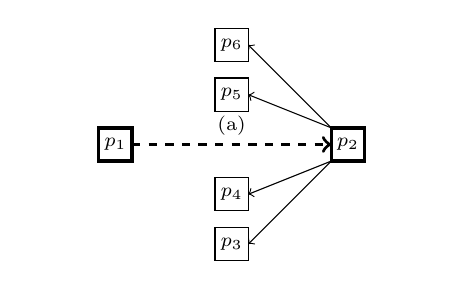
\begin{tikzpicture}[scale=1.2]

  \newcommand\X{35pt};
  \newcommand\Y{15pt};

  \draw(-0.75*\X, 0pt); %% positioning
  \draw( 2.75*\X, 0pt); %% positioning

  \scriptsize
  \draw[->,dashed,very thick](5+0*\X, 0*\Y) -- 
  node[anchor=south]{(a)}(-5+ 2*\X, 0*\Y);
  \draw[->] (-5+2*\X, 5pt) -- (5+\X, \Y);
  \draw[->] (-5+2*\X, 5pt) --  (5+\X, 2*\Y);
  \draw[->] (-5+2*\X, -5pt) -- (5+\X, -\Y);
  \draw[->] (-5+2*\X, -5pt) -- (5+\X, -2*\Y);

  \draw[fill=white, very thick]
  (0*\X, 0*\Y) node{$p_1$} +(-5pt,-5pt) rectangle +(5pt,5pt);
  \draw[fill=white, very thick]
  (2*\X, 0*\Y) node{$p_2$} +(-5pt,-5pt) rectangle +(5pt,5pt);

  \draw[fill=white](1*\X,2*\Y) node{$p_6$} +(-5pt,-5pt) rectangle +(5pt,5pt);
  \draw[fill=white](1*\X,1*\Y) node{$p_5$} +(-5pt,-5pt) rectangle +(5pt,5pt);
  \draw[fill=white](1*\X,-1*\Y) node{$p_4$} +(-5pt,-5pt) rectangle +(5pt,5pt);
  \draw[fill=white](1*\X,-2*\Y) node{$p_3$} +(-5pt,-5pt) rectangle +(5pt,5pt);
  
\end{tikzpicture}}
  \hspace{8pt}
  \subfloat[Figure B][The $onSubs(p_1)$ event is raised at $p_1$
  which forwards the subscription to $p_1$'s neighborhood.]{
    
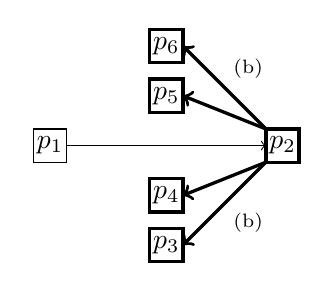
\begin{tikzpicture}[scale=1.2]

  \newcommand\X{35pt};
  \newcommand\Y{15pt};

  \scriptsize
  \draw[->](5+0*\X, 0*\Y) -- (-5+ 2*\X, 0*\Y);
  \draw[->, very thick] (-5+2*\X, 5pt) -- (5+\X, \Y);
  \draw[->, very thick] (-5+2*\X, 5pt) --
  node[anchor=south west]{(b)} (5+\X, 2*\Y);
  \draw[->, very thick] (-5+2*\X, -5pt) -- (5+\X, -\Y);
  \draw[->, very thick] (-5+2*\X, -5pt) --
  node[anchor=north west]{(b)}(5+\X, -2*\Y);

  \normalsize
  \draw[fill=white]
  (0*\X, 0*\Y) node{$p_1$} +(-5pt,-5pt) rectangle +(5pt,5pt);
  \draw[fill=white, very thick]
  (2*\X, 0*\Y) node{$p_2$} +(-5pt,-5pt) rectangle +(5pt,5pt);

  \draw[fill=white, very thick]
  (1*\X,2*\Y) node{$p_6$} +(-5pt,-5pt) rectangle +(5pt,5pt);
  \draw[fill=white, very thick]
  (1*\X,1*\Y) node{$p_5$} +(-5pt,-5pt) rectangle +(5pt,5pt);
  \draw[fill=white, very thick]
  (1*\X,-1*\Y) node{$p_4$} +(-5pt,-5pt) rectangle +(5pt,5pt);
  \draw[fill=white, very thick]
  (1*\X,-2*\Y) node{$p_3$} +(-5pt,-5pt) rectangle +(5pt,5pt);

\end{tikzpicture}}
  \hspace{8pt}
  \subfloat[Figure C][The $onFwdSubs(p_1)$ event is raised at $p_{3-6}$. The 
  peers add $p_1$ to their neighborhood.]{
    
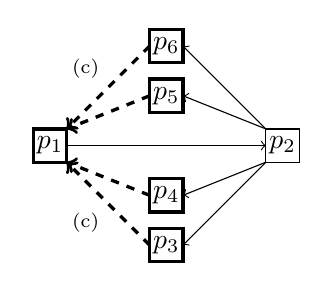
\begin{tikzpicture}[scale=1.2]

  \newcommand\X{35pt};
  \newcommand\Y{15pt};

  \scriptsize
  \draw[->](5+0*\X, 0*\Y) -- (-5+ 2*\X, 0*\Y);
  \draw[->] (-5+2*\X, 5pt) -- (5+\X, \Y);
  \draw[->] (-5+2*\X, 5pt) -- (5+\X, 2*\Y);
  \draw[->] (-5+2*\X, -5pt) -- (5+\X, -\Y);
  \draw[->] (-5+2*\X, -5pt) -- (5+\X, -2*\Y);

  \draw[->,dashed, very thick](-5+\X, 2*\Y) --
  node[anchor=south east]{(c)} ( 5pt,5pt);
  \draw[->,dashed, very thick](-5+\X, 1*\Y) -- ( 5pt,5pt);
  \draw[->,dashed, very thick](-5+\X, -1*\Y) -- ( 5pt,-5pt);
  \draw[->,dashed, very thick](-5+\X, -2*\Y) --
  node[anchor=north east]{(c)}( 5pt,-5pt);

  \normalsize
  \draw[fill=white, very thick]
  (0*\X, 0*\Y) node{$p_1$} +(-5pt,-5pt) rectangle +(5pt,5pt);
  \draw[fill=white]
  (2*\X, 0*\Y) node{$p_2$} +(-5pt,-5pt) rectangle +(5pt,5pt);

  \draw[fill=white, very thick]
  (1*\X,2*\Y) node{$p_6$} +(-5pt,-5pt) rectangle +(5pt,5pt);
  \draw[fill=white, very thick]
  (1*\X,1*\Y) node{$p_5$} +(-5pt,-5pt) rectangle +(5pt,5pt);
  \draw[fill=white, very thick]
  (1*\X,-1*\Y) node{$p_4$} +(-5pt,-5pt) rectangle +(5pt,5pt);
  \draw[fill=white, very thick]
  (1*\X,-2*\Y) node{$p_3$} +(-5pt,-5pt) rectangle +(5pt,5pt);
 

\end{tikzpicture}}
  \caption{\label{fig:joiningexample}Example of the \SPRAY's joining
    protocol.}
\end{figure*}

The sole representative of adaptive-by-design random peer sampling is
\SCAMP~\cite{ganesh2003peer}. Its interesting property lies in
its logarithmically growing partial view sizes meeting the sharp threshold of
connectedness of random graphs~\cite{erdos1959random}. Nevertheless, \SCAMP
suffers from other drawbacks. In particular, it systematically disseminates the
connections at random. Thus, the originating peer can be several hops away from
the arrival peer. In WebRTC, each random dissemination path must be traveled
back to finalize the connection establishment
(cf. Figure~\ref{fig:webrtc}). This drastically impacts the \SCAMP failure
probability of establishing a connection. In turns, the number of connections
quickly decreases eventually leading to partitioning.

%  Let $P_f$ be the probability that an
% element of the dissemination path (either a peer or a connection) crashes or
% leaves during a hop of the three-way handshake, without any possible
% recovery. Let $P_E$ be the probability that a connection establishment cannot
% be completed. Without three-way handshake, $P_E$ is straightforward:
% \begin{equation} P_{E,\,1way}^{Scamp}=1-(1- P_f)^{k+1} \end{equation} This
% corresponds to the probability that each element (arc and peer) in the path of
% size $k+1$ stays alive during their part of the dissemination (i.e., otherwise,
% they are allowed to crash or leave). In the context of WebRTC, the offer ticket must
% travel back to its emitter. As a consequence, the elements of the random
% dissemination path are not allowed to fail until the stamped ticket travels
% back. We obtain:
% \begin{align} P_{E,\,3way}^{Scamp} &=1 - ((1-P_f)^{2(k+1)} (1-P_f)^{2k}
%                                      \ldots (1-P_f)^2) \nonumber \\
%                                    &=1-(1-P_f)^{k^2+3k+2}
% \end{align}
% In other terms, the first chosen arc and peer in the path must stay alive
% $2k+2$ hops, the second chosen arc and peer must stay alive $2k$ hops etc.  The
% complexity class of the \SCAMP failure rate increases leading to a quicker
% degeneration of the connection count. This behavior endangers the network
% connectedness.%%, as depicted in Section~\ref{subsec:degeneration}.

Building an adaptive-by-design random peer sampling that meets WebRTC
constraints raises the following scientific problem:
\begin{problem}
  Let $t$ be an arbitrary time frame, let $\mathcal{N}^t$ be the network
  membership at that given time $t$ and let $\mathcal{P}_x^t$ be the partial
  view of peer $p_x \in \mathcal{N}^t$.  A cost-efficient random peer sampling
  should provide the following best-case properties:
  \begin{enumerate}
  \item Partial view size: \hfill
    $\forall p_x \in \mathcal{N}^t,\, |\mathcal{P}_x^t| = \Theta (\ln
    |\mathcal{N}^t|)$      
  \item Connection establishment: \hfill $O(1)$
    %% \item  \begin{center}
    %%     Convergence speed: \hfill $\Theta(\exp \, t^{-1})$
    %%   \end{center}
  \end{enumerate}
\end{problem}

The first condition states that the partial view size is relative to the size
of the network at any time. It also states that partial views grow and shrink
logarithmically compared to the size of the network. The second condition
states that each connection establishment requires a constant number of
intermediary peers. Since this number is constant, connection establishments
do not depend on the network size.
%% The last condition states that the network
%% overlay converges exponentially fast to a topology that is close to a random
%% graph.
Lpbcast, HyParView, Newscast, and \CYCLON fail to meet the first condition of
the problem statement since they do not adapt their views to the network
size. \SCAMP fails to meet the second condition of the problem statement since
each connection implies an unsafe random dissemination protocol.

%%% Local Variables:
%%% mode: latex
%%% TeX-master: "../paper"
%%% End:


\section{Spray}
\label{sec:proposal}

\SCAMPLON{} \SCAMPLONDESCRIPTION{} is an adaptive random peer sampling protocol
inspired by \SCAMP{}~\cite{ganesh2003peer} and
\CYCLON{}~\cite{voulgaris2005cyclon}. It comprises three parts representing the
lifecycle of a peer in the network.  Firstly, the joining process injects a
logarithmically growing number of arcs in the network. Hence, the number of
arcs scales with the network size.  Nevertheless, the resulting overlay has
flaws. Consequently, each peer runs a periodic process in order to balance the
partial views both in terms of partial view size, and uniformity of the
referenced peers within them. Quickly, the overlay network converges to a
topology exposing properties of the random graphs. Finally, A peer is able to
leave at any time without giving notice (equivalent to a crash), still the
network properties do not degrade.

\subsection{Joining}

The main focus of the joining protocol is about establishing a logarithmically
growing number of arcs in the network compared to the number of members.
\SCAMPLON{} assumes that each peer has a logarithmic partial view size. Thus,
when a peer $p_1$ contacts a peer $p_2$ within the network, Peer $p_2$ is able
to use its partial view size to spread the appropriate number of subscriptions.
Peer $p_2$ simply forwards the identity of $p_1$ to the latter's neighbors
where they directly add it to their partial view. Afterwards, $p_1$ is
connected to $p_2$, and all the neighbors of $p_2$ are connected to $p_1$. The
total number of connections in the network gently increases of
$1+\ln(|\mathcal{N}|)$.

\begin{algorithm}[h]

\small
\SetKwProg{Function}{function}{}{}
\SetKwProg{INITIALLY}{INITIALLY}{}{}
\SetKwProg{EVENTS}{EVENTS}{}{}
\DontPrintSemicolon
\LinesNumbered

\INITIALLY {} {
  $\mathcal{P} \leftarrow \varnothing$ \Comment{the partial view is a multiset} \;
}

\EVENTS {} {
  \Function{onSubs($o$)} { % \hfill \comm{$o: origin$}
    \lFor{\textbf{each} $\langle q,\,\_\, \rangle \in\mathcal{P}$}
    {$sendTo(q,\, 'fwdSubs',\, o)$} \label{line:multicast}
  }

  \BlankLine

  \Function{onFwdSubs($o$)} {% \hfill \comm{$o: origin$}
    $\mathcal{P} \leftarrow \mathcal{P}\uplus \left\{\langle o,\, 0 \rangle\right\}$
  }

}

\caption{\label{algo:joiningalgo}The joining protocol of \SCAMPLON{}.}
\end{algorithm}

Algorithm~\ref{algo:joiningalgo} shows the simplicity of this joining
protocol. First, the partial view $\mathcal{P}$ is a multiset of pairs
$\langle n,\, age\rangle$ which associate to the neighbor $n$ the age $age$
(the age is useful in the periodic protocol). Thus, a neighbor can appear
multiple times in the partial view. Second, the algorithm shows the $onSubs$
event called each time a peer joins the network which simply forwards the
identity of the joining peer to all neighbors, indifferently of the age. The
$onFwdSubs$ event is called when a peer receives such forwarded
subscription. It adds the peer as one of its neighbor with an age set to $0$
meaning that it is a brand new connection.

\begin{figure*}
  \centering
  \subfloat[Figure A][Subscription]{
    
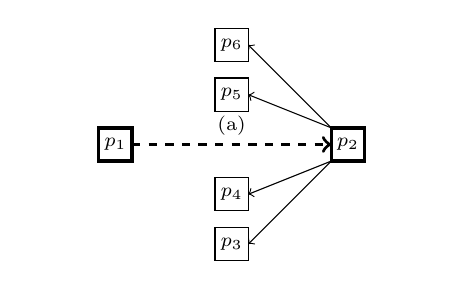
\begin{tikzpicture}[scale=1.2]

  \newcommand\X{35pt};
  \newcommand\Y{15pt};

  \draw(-0.75*\X, 0pt); %% positioning
  \draw( 2.75*\X, 0pt); %% positioning

  \scriptsize
  \draw[->,dashed,very thick](5+0*\X, 0*\Y) -- 
  node[anchor=south]{(a)}(-5+ 2*\X, 0*\Y);
  \draw[->] (-5+2*\X, 5pt) -- (5+\X, \Y);
  \draw[->] (-5+2*\X, 5pt) --  (5+\X, 2*\Y);
  \draw[->] (-5+2*\X, -5pt) -- (5+\X, -\Y);
  \draw[->] (-5+2*\X, -5pt) -- (5+\X, -2*\Y);

  \draw[fill=white, very thick]
  (0*\X, 0*\Y) node{$p_1$} +(-5pt,-5pt) rectangle +(5pt,5pt);
  \draw[fill=white, very thick]
  (2*\X, 0*\Y) node{$p_2$} +(-5pt,-5pt) rectangle +(5pt,5pt);

  \draw[fill=white](1*\X,2*\Y) node{$p_6$} +(-5pt,-5pt) rectangle +(5pt,5pt);
  \draw[fill=white](1*\X,1*\Y) node{$p_5$} +(-5pt,-5pt) rectangle +(5pt,5pt);
  \draw[fill=white](1*\X,-1*\Y) node{$p_4$} +(-5pt,-5pt) rectangle +(5pt,5pt);
  \draw[fill=white](1*\X,-2*\Y) node{$p_3$} +(-5pt,-5pt) rectangle +(5pt,5pt);
  
\end{tikzpicture}}
  \hspace{40pt}
  \subfloat[Figure B][Forwarding]{
    
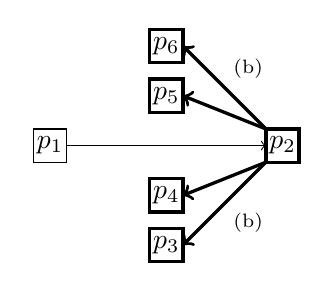
\begin{tikzpicture}[scale=1.2]

  \newcommand\X{35pt};
  \newcommand\Y{15pt};

  \scriptsize
  \draw[->](5+0*\X, 0*\Y) -- (-5+ 2*\X, 0*\Y);
  \draw[->, very thick] (-5+2*\X, 5pt) -- (5+\X, \Y);
  \draw[->, very thick] (-5+2*\X, 5pt) --
  node[anchor=south west]{(b)} (5+\X, 2*\Y);
  \draw[->, very thick] (-5+2*\X, -5pt) -- (5+\X, -\Y);
  \draw[->, very thick] (-5+2*\X, -5pt) --
  node[anchor=north west]{(b)}(5+\X, -2*\Y);

  \normalsize
  \draw[fill=white]
  (0*\X, 0*\Y) node{$p_1$} +(-5pt,-5pt) rectangle +(5pt,5pt);
  \draw[fill=white, very thick]
  (2*\X, 0*\Y) node{$p_2$} +(-5pt,-5pt) rectangle +(5pt,5pt);

  \draw[fill=white, very thick]
  (1*\X,2*\Y) node{$p_6$} +(-5pt,-5pt) rectangle +(5pt,5pt);
  \draw[fill=white, very thick]
  (1*\X,1*\Y) node{$p_5$} +(-5pt,-5pt) rectangle +(5pt,5pt);
  \draw[fill=white, very thick]
  (1*\X,-1*\Y) node{$p_4$} +(-5pt,-5pt) rectangle +(5pt,5pt);
  \draw[fill=white, very thick]
  (1*\X,-2*\Y) node{$p_3$} +(-5pt,-5pt) rectangle +(5pt,5pt);

\end{tikzpicture}}
  \hspace{40pt}
  \subfloat[Figure C][Connections]{
    
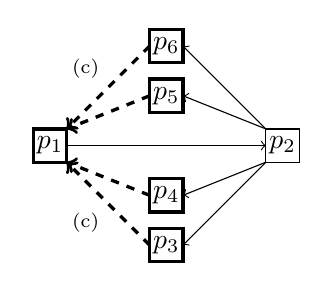
\begin{tikzpicture}[scale=1.2]

  \newcommand\X{35pt};
  \newcommand\Y{15pt};

  \scriptsize
  \draw[->](5+0*\X, 0*\Y) -- (-5+ 2*\X, 0*\Y);
  \draw[->] (-5+2*\X, 5pt) -- (5+\X, \Y);
  \draw[->] (-5+2*\X, 5pt) -- (5+\X, 2*\Y);
  \draw[->] (-5+2*\X, -5pt) -- (5+\X, -\Y);
  \draw[->] (-5+2*\X, -5pt) -- (5+\X, -2*\Y);

  \draw[->,dashed, very thick](-5+\X, 2*\Y) --
  node[anchor=south east]{(c)} ( 5pt,5pt);
  \draw[->,dashed, very thick](-5+\X, 1*\Y) -- ( 5pt,5pt);
  \draw[->,dashed, very thick](-5+\X, -1*\Y) -- ( 5pt,-5pt);
  \draw[->,dashed, very thick](-5+\X, -2*\Y) --
  node[anchor=north east]{(c)}( 5pt,-5pt);

  \normalsize
  \draw[fill=white, very thick]
  (0*\X, 0*\Y) node{$p_1$} +(-5pt,-5pt) rectangle +(5pt,5pt);
  \draw[fill=white]
  (2*\X, 0*\Y) node{$p_2$} +(-5pt,-5pt) rectangle +(5pt,5pt);

  \draw[fill=white, very thick]
  (1*\X,2*\Y) node{$p_6$} +(-5pt,-5pt) rectangle +(5pt,5pt);
  \draw[fill=white, very thick]
  (1*\X,1*\Y) node{$p_5$} +(-5pt,-5pt) rectangle +(5pt,5pt);
  \draw[fill=white, very thick]
  (1*\X,-1*\Y) node{$p_4$} +(-5pt,-5pt) rectangle +(5pt,5pt);
  \draw[fill=white, very thick]
  (1*\X,-2*\Y) node{$p_3$} +(-5pt,-5pt) rectangle +(5pt,5pt);
 

\end{tikzpicture}}
  \caption{\label{fig:joiningexample}Example of the \SCAMPLON{}'s joining
    protocol. In this scenario, Peer $p_1$ contacts $p_2$ to join the network
    composed of $\{p_2,\,p_3,\,p_4,\,p_5,\,p_6\}$ (for simplicity sake, only
    the new connections and the neighborhood of $p_1$ and $p_2$ are
    displayed). Peer $p_1$ directly adds $p_2$ in its partial view. Peer $p_2$
    forwards the identity of $p_1$ to its neighborhood. Each of these neighbors
    adds $p_1$ in their partial view. Five connections have been established.}
\end{figure*}

Figure~\ref{fig:joiningexample} depicts a joining scenario. Although the
joining peer is connected to the network, the example shows that the network
topology is not ideal after a joining protocol. Indeed, the joining peer only
has one neighbor in its partial view, and all the neighbors of this neighbor
have the joining peer in their partial view. Consequently, the network is not
robust and highly clustered. Churn puts the connectedness at risk. To avoid it,
\SCAMPLON{} needs a balancing protocol.

\subsection{Cyclic}
\label{subsec:cyclic}

\SCAMPLON{} is a random peer sampling protocol. As such, it must constantly
renew the connections to handle the churn (when peers join and leave freely).
To ensure this constant shuffling, \SCAMPLON{} repeats an exchanging procedure
during which two peers swap their neighbors. The swapping aims to balance both
the size of partial views and the global distribution of peers among them.

\SCAMPLON{} uses a multiset as partial view without any predefined boundary on
its size. Thus, two peers with different partial view sizes can swap their
neighbors, the objective being that both peers become as connected as one
another. The global number of connections and the connectedness must remain
unchanged.

\SCAMPLON{} converges to the ideal partial view size by averaging their size
over exchanges. Therefore, both peers involved send and integrate
$\left\lceil|\mathcal{P}|\over{2}\right\rceil$ neighbors from each
other. Since the partial views are multisets, even if a neighbor appears
multiple times, the network does not lose any connection. It guarantees that
the global number of connections after the protocol does not change.

\begin{algorithm}[h] %% to change if repositionning possible
  
\small
\algrenewcommand{\algorithmiccomment}[1]{\hskip2em$\rhd$ #1}

\newcommand{\comm}[1]{$\rhd$ #1}

\algblockdefx[act]{act}{endAct}
  [0] {\textbf{ACTIVE THREAD:}}

\algsetblockdefx[pas]{pas}{endPas}
{65535}{}
[0] {\textbf{PASSIVE THREAD:}}


\newcommand{\LINEFOR}[2]{%
  \algorithmicfor\ {#1}\ \algorithmicdo\ {#2} %
  }

\newcommand{\LINEIFTHEN}[2]{%
  \algorithmicif\ {#1}\ \algorithmicthen\ {#2} %
  }

\newcommand{\INDSTATE}[1][1]{\State\hspace{\algorithmicindent}}

\begin{algorithmic}[1]
  \Statex
  \act
    \Function{loop}{ } \hfill \comm{Every $\Delta\,t$}
    \State $\mathcal{P} \leftarrow incrementAge(\mathcal{P})$;
    \State \textbf{let} $ \langle q,\, age \rangle \leftarrow getOldest(\mathcal{P})$;
    \State \textbf{let} $sample \leftarrow $ \label{line:samplesize}
    \Statex \hfill $getSample(\mathcal{P}\setminus\left\{\langle q, age\rangle\right\}, \left \lceil{|\mathcal{P}|\over{2}} \right \rceil-1) \uplus \left\{\langle p, 0 \rangle\right\}$;
    \State $sample \leftarrow replace(sample,\,q,\,p)$; \label{line:replace1}
    \State $sendTo(q,\, 'exchange',\, sample)$;
    \State \textbf{let} $sample'\leftarrow receiveFrom(q)$;
    \State $sample \leftarrow replace(sample,\,p,\,q)$;
    \State $\mathcal{P} \leftarrow (\mathcal{P} \setminus sample) \uplus
    sample'$;
    \EndFunction
  \endAct
  
  \pas
    \Function{onExchange}{$o,\, sample$} \hfill \comm{$o: origin$}
    \State \textbf{let} $sample' \leftarrow getSample(\mathcal{P} ,\, \left\lceil |\mathcal{P}|\over{2} \right\rceil )$;
    \State $sample' \leftarrow replace(sample',\,o,\,p);$ \label{line:replace2}
    \State $sendTo(o ,\, sample')$;
    \State $sample' \leftarrow replace(sample',\,p,\,o)$;
    \State $\mathcal{P} \leftarrow (\mathcal{P} \setminus sample') \uplus
    sample$; 
    \EndFunction
%%  \endPas
  
\end{algorithmic}

  \caption{\label{algo:scamplon}The cyclic protocol of \SCAMPLON{}.}
\end{algorithm}

There exists a close relationship between \SCAMPLON{} and the proactive
aggregation protocol introduced
in~\cite{jelasity2004epidemic,montresor2004robust}. The latter states that,
under the assumption of a peer sampling sufficiently random, the mean value
$\mu$ and the variance $\sigma^2$ at a given cycle $i$ are:
\begin{center}
  $\mu_i = {1\over{|\mathcal{N}|}} \sum\limits_{x \in \mathcal{N}} a_{i,\,x}$
  \hfill
  $\sigma^2_i = {1\over{|\mathcal{N}|-1}}\sum\limits_{x \in \mathcal{N}}
  (a_{i,\,x} - \mu_i)^2$
\end{center}
where $a_{i,\,x}$ is the value held by Peer $p_x$ at cycle $i$. The estimated
variance must converge to $0$ over cycles. In other terms, the values tends to
be the same over cycles. In the \SCAMPLON{} case, the value $a_{i,\,x}$ is the
partial view size of Peer $p_x$ at cycle $i$. Indeed, each exchange from Peer
$p_1$ to Peer $p_2$ is an aggregation resulting to:
$|\mathcal{P}_1|\approx|\mathcal{P}_2|\approx{|\mathcal{P}_1| + |\mathcal{P}_2|
  \over{2}}$.
Furthermore, at each cycle, each peer is involved in the exchange protocol at
least once (they initiate one), and in the best case 1+Poisson(1) (they
initiate one and, in average, each peer receives another one). This
relation being established, we know that \SCAMPLON{} converges exponentially
fast. Furthermore, we know that each cycle decreases the variance of the
overall system at a rate comprised between ${1\over{2}}$ and
$1\over{2\sqrt{\text{e}}}$.


\begin{figure*}
  \centering
  \subfloat[Figure A]
  [Peer $p_6$ initiates the exchange with $p_1$ by sending to the
  latter the multiset $\{p_6,\,p_9\}$.]{
    
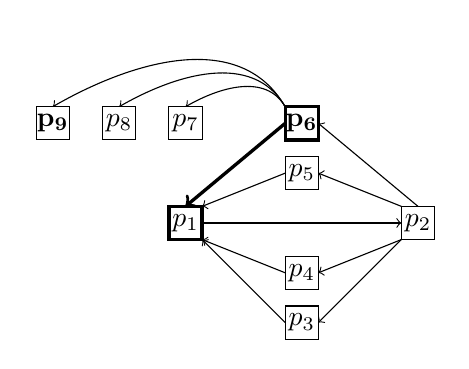
\begin{tikzpicture}[scale=1.2]

  \newcommand\X{35pt};
  \newcommand\Y{15pt};

  \draw[->](5+0*\X, 0*\Y) -- (-5+ 2*\X, 0*\Y); %% 1 -> 2
  \draw[->] (-5+2*\X, 5pt) -- (5+\X, \Y);
  \draw[->](2*\X,5pt) -- (5+1*\X, 2*\Y); %% 2 -> 6
  \draw[->] (-5+2*\X, -5pt) -- (5+\X, -\Y);
  \draw[->] (-5+2*\X, -5pt) -- (5+\X, -2*\Y);

  \draw[->,very thick](-5+\X,2*\Y) -- (0pt,5pt); %% 6 -> 1

  \draw[->](-5+\X, 1*\Y) -- ( 5pt,5pt);
  \draw[->](-5+\X, -1*\Y) -- ( 5pt,-5pt);
  \draw[->](-5+\X, -2*\Y) -- ( 5pt,-5pt);

  \draw[->](-5+\X, 5+2*\Y)to[out=120,in=30](0pt,5+2*\Y); %% 6 -> 7
  \draw[->](-5+\X, 5+2*\Y)to[out=120,in=30](-5-\Y ,5+2*\Y); %% 6 -> 8
  \draw[->](-5+\X, 5+2*\Y)to[out=120,in=30](-10-2*\Y,5+2*\Y); %% 6 -> 9

  \normalsize
  \draw[fill=white, very thick]
  (0*\X, 0*\Y) node{$p_1$} +(-5pt,-5pt) rectangle +(5pt,5pt);
  \draw[fill=white](2*\X, 0*\Y) node{$p_2$} +(-5pt,-5pt) rectangle +(5pt,5pt);

  \draw[fill=white,very thick]
  (1*\X,2*\Y) node{$\mathbf{p_6}$} +(-5pt,-5pt) rectangle +(5pt,5pt);
  \draw[fill=white](1*\X,1*\Y) node{$p_5$} +(-5pt,-5pt) rectangle +(5pt,5pt);
  \draw[fill=white](1*\X,-1*\Y) node{$p_4$} +(-5pt,-5pt) rectangle +(5pt,5pt);
  \draw[fill=white](1*\X,-2*\Y) node{$p_3$} +(-5pt,-5pt) rectangle +(5pt,5pt);

  \draw[fill=white]( 0*\X,2*\Y)
  node{$p_7$} +(-5pt,-5pt) rectangle +(5pt,5pt);
  \draw[fill=white](-5+-\Y,2*\Y)node{$p_8$} +(-5pt,-5pt) rectangle +(5pt,5pt);
  \draw[fill=white](-10+-2*\Y,2*\Y) node{$\mathbf{p_9}$} +(-5pt,-5pt) rectangle +(5pt,5pt);
  

\end{tikzpicture}}
  \hspace{10pt}
  \subfloat[Figure B][Peer $p_1$ receives the $p_6$'s message. 
  It sends back the multiset $\{p_2\}$ and adds $\{p_6,\,p_9\}$ to its 
  partial view.]{
    
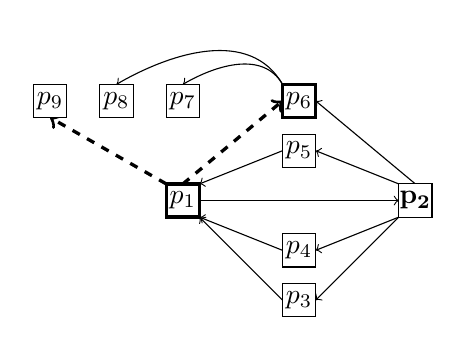
\begin{tikzpicture}[scale=1.2]

  \newcommand\X{35pt};
  \newcommand\Y{15pt};

  \draw[->](5+0*\X, 0*\Y) -- (-5+ 2*\X, 0*\Y); %% 1 -> 2
  \draw[->] (-5+2*\X, 5pt) -- (5+\X, \Y);
  \draw[->](2*\X,5pt) -- (5+1*\X, 2*\Y); %% 2 -> 6
  \draw[->] (-5+2*\X, -5pt) -- (5+\X, -\Y);
  \draw[->] (-5+2*\X, -5pt) -- (5+\X, -2*\Y);

  \draw[->,dashed, very thick](0pt,5pt)--(-5+\X, 2*\Y); %% 1 -> 6

  \draw[->](-5+\X, 1*\Y) -- ( 5pt,5pt);
  \draw[->](-5+\X, -1*\Y) -- ( 5pt,-5pt);
  \draw[->](-5+\X, -2*\Y) -- ( 5pt,-5pt);

  \draw[->](-5+\X, 5+2*\Y)to[out=120,in=30](0pt,5+2*\Y); %% 6 -> 7
  \draw[->](-5+\X, 5+2*\Y)to[out=120,in=30](-5-\Y ,5+2*\Y); %% 6 -> 8
  
  \draw[->,dashed, very thick](-5pt,5pt)--(-10-2*\Y,-5+2*\Y); %% 1 -> 9

  \normalsize
  \draw[fill=white, very thick]
  (0*\X, 0*\Y) node{$p_1$} +(-5pt,-5pt) rectangle +(5pt,5pt);
  \draw[fill=white](2*\X, 0*\Y)
  node{$\mathbf{p_2}$} +(-5pt,-5pt) rectangle +(5pt,5pt);

  \draw[fill=white,very thick]
  (1*\X,2*\Y) node{$p_6$} +(-5pt,-5pt) rectangle +(5pt,5pt);
  \draw[fill=white](1*\X,1*\Y) node{$p_5$} +(-5pt,-5pt) rectangle +(5pt,5pt);
  \draw[fill=white](1*\X,-1*\Y) node{$p_4$} +(-5pt,-5pt) rectangle +(5pt,5pt);
  \draw[fill=white](1*\X,-2*\Y) node{$p_3$} +(-5pt,-5pt) rectangle +(5pt,5pt);

  \draw[fill=white]( 0*\X,2*\Y)
  node{$p_7$} +(-5pt,-5pt) rectangle +(5pt,5pt);
  \draw[fill=white](-5+-\Y,2*\Y)node{$p_8$} +(-5pt,-5pt) rectangle +(5pt,5pt);
  \draw[fill=white](-10+-2*\Y,2*\Y) node{$p_9$} +(-5pt,-5pt) rectangle +(5pt,5pt);
  

\end{tikzpicture}}
  \hspace{10pt}
  \subfloat[Figure C][Peer $p_6$ receives the $p_1$'s response, it
  adds $\{p_2\}$ to its partial view.]{
    
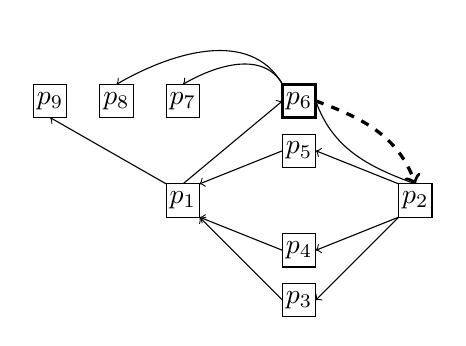
\begin{tikzpicture}[scale=1.2]

  \newcommand\X{35pt};
  \newcommand\Y{15pt};

  \draw[->] (-5+2*\X, 5pt) -- (5+\X, \Y);
  \draw[->,dashed, very thick]
  (5+\X, 2*\Y)to[out=-20,in=110](2*\X, 5pt); %% 6 -> 2
  \draw[->](2*\X,5pt)to[out=160,in=-70](5+1*\X, 2*\Y); %% 2 -> 6
  \draw[->] (-5+2*\X, -5pt) -- (5+\X, -\Y);
  \draw[->] (-5+2*\X, -5pt) -- (5+\X, -2*\Y);

  \draw[->](0pt,5pt)--(-5+\X, 2*\Y); %% 1 -> 6

  \draw[->](-5+\X, 1*\Y) -- ( 5pt,5pt);
  \draw[->](-5+\X, -1*\Y) -- ( 5pt,-5pt);
  \draw[->](-5+\X, -2*\Y) -- ( 5pt,-5pt);

  \draw[->](-5+\X, 5+2*\Y)to[out=120,in=30](0pt,5+2*\Y); %% 6 -> 7
  \draw[->](-5+\X, 5+2*\Y)to[out=120,in=30](-5-\Y ,5+2*\Y); %% 6 -> 8
  
  \draw[->](-5pt,5pt)--(-10-2*\Y,-5+2*\Y); %% 1 -> 9

  \normalsize
  \draw[fill=white]
  (0*\X, 0*\Y) node{$p_1$} +(-5pt,-5pt) rectangle +(5pt,5pt);
  \draw[fill=white](2*\X, 0*\Y) node{$p_2$} +(-5pt,-5pt) rectangle +(5pt,5pt);

  \draw[fill=white,very thick]
  (1*\X,2*\Y) node{$p_6$} +(-5pt,-5pt) rectangle +(5pt,5pt);
  \draw[fill=white](1*\X,1*\Y) node{$p_5$} +(-5pt,-5pt) rectangle +(5pt,5pt);
  \draw[fill=white](1*\X,-1*\Y) node{$p_4$} +(-5pt,-5pt) rectangle +(5pt,5pt);
  \draw[fill=white](1*\X,-2*\Y) node{$p_3$} +(-5pt,-5pt) rectangle +(5pt,5pt);

  \draw[fill=white]( 0*\X,2*\Y)
  node{$p_7$} +(-5pt,-5pt) rectangle +(5pt,5pt);
  \draw[fill=white](-5+-\Y,2*\Y)node{$p_8$} +(-5pt,-5pt) rectangle +(5pt,5pt);
  \draw[fill=white](-10+-2*\Y,2*\Y) node{$p_9$} +(-5pt,-5pt) rectangle +(5pt,5pt);
  

\end{tikzpicture}}
  \caption{\label{fig:cyclicexample}Example of the \SCAMPLON{}'s cyclic
    protocol. This scenario follows from Figure~\ref{fig:joiningexample}: Peer
    $p_1$ just joined the network. Peer $p_6$ initiates an exchange with $p_1$
    (the oldest among the $p_6$'s partial view). It randomly chooses
    $\left\lceil{|\mathcal{P}_6|\over{2}}\right\rceil-1 = 1$ peer among its
    neighborhood. In this case, it picks $p_9$ from $\{p_9,\,p_8,\,p_7\}$.  It
    sends the chosen peer plus its own identity to Peer $p_1$. In response, the
    latter picks $\left\lceil{|\mathcal{P}_1|\over{2}}\right\rceil = 1$ peer
    from its partial view. It sends back its sole neighbor $p_2$ and directly
    adds the received neighbor to its partial view. After receipt, Peer $p_6$
    removes the sent neighbors from its partial view, removes an occurrence of
    $p_1$, and adds the received peer from $p_1$. The peers $\{p_6,\,p_9\}$
    compose the $p_1$'s partial view. The peers $\{p_2,\,p_7,\,p_8\}$ compose
    the $p_6$'s partial view.}
\end{figure*}


Algorithm~\ref{algo:scamplon} shows the \SCAMPLON{} protocol running at each
peer. It is divided between an active thread looping to update the partial
view, and a passive thread which reacts to an exchange message. The functions
which are not explicitly defined are the following:
\begin{itemize}
\item $incrementAge(view)$: increments the age of each elements in the view
  and returns the modified view.
\item $getOldest(view)$: retrieves the oldest of peers contained in the view.
\item $getSample(view, \, size)$: returns a sample of the view containing
  $size$ elements.
\item $replace(view,\,old,\,new)$: replaces in the view all occurrences of
  the $old$ element by the $new$ element and returns the modified view.
\item $rand()$: generates a random floating number between $0$ and $1$.
\end{itemize}
In the active thread, Function $loop$ is called every $\Delta$ time
$t$. Firstly, the function increments the age of each neighbor in
$\mathcal{P}$. Then, the oldest peer $q$ is chosen to exchange a subset of its
partial view. If Peer $q$ cannot be reached (i.e. it crashed/left), the peer
$p$ executes the crash handling function (cf. Section~\ref{subsec:leaving}) and
repeats the process until it finds a reachable peer $q$. Peer $p$ selects a
sample of its partial view, excluding one occurrence of $q$ and including
itself. The size of this sample is half of its partial view, with at least one
peer: the initiating peer (cf. Line~\ref{line:samplesize}). The answer of $q$
contains half of its partial view too. Since peers can appear multiple times in
$\mathcal{P}$, the exchanging peers may send references to the other peer,
e.g., Peer $o$'s sample can contain references to $q$. Such sample, without
further processing, would create self-loop ($q$'s partial view contains
references to $q$). To alleviate this undesirable behavior, all occurrences of
the other peer are replaced with the emitting peer
(cf. Line~\ref{line:replace1},~\ref{line:replace2}).  Afterwards, both of
them remove the sent sample from their view and add the received
sample. Additionally, the initiating peer removes an occurrence of the chosen
peer $q$.



Figure~\ref{fig:cyclicexample} depicts the \SCAMPLON{}'s cyclic procedure. The
example shows that, at first, the initiating peer has $4$ peers in its partial
view, while the receiving peer has only $1$ peer. Then, after the exchange, the
former has $3$ neighbors including $1$ new peer. The receiving peer has $2$
neighbors, and both of them are new. Thus, the periodic procedure tends to
even up the partial view size of network members. It also scatters neighbors in
order to remove the highly clustered groups which may appear because of the
joining protocol.

\subsection{Leaving}
\label{subsec:leaving}

Using \SCAMPLON{}, the peers are free to leave the network without giving
notice. In that regard, we do not consider the departures and the crashs
differently.  Without any appropriate reaction, the network may collapse due to
an over zealous removal of connections. Indeed, when a peer joins the network,
it injects in it $1+\ln(|\mathcal{N}|)$ connections. Nevertheless, after few
exchanges, the partial view of the joining peer becomes populated with more
neighbors. Then, if this peer leaves, it removes $\ln(|\mathcal{N}|)$
connections from its partial view, and another $\ln(|\mathcal{N}|)$ connections
from peers which have this peer in their partial view. Therefore, without any
crash handler, we remove $2\ln(|\mathcal{N}|)$ connections instead of
$1+\ln(|\mathcal{N}|)$. To alleviate this issue, each peer that detects a crash
may reestablish a connection with anyone in its neighborhood (which will spread
in the network over the exchanges). The probability of reestablishing a
connection is $1-{1\over{|\mathcal{P}|}}$. Since
${|\mathcal{P}|}\approx \ln(|\mathcal{N}|)$ peers have the crashed peer in
their partial view, it is likely that all of them will reestablish a
connection, excepted one. Therefore, when a peer leaves, it approximately
removes the number of connections it injected when it joined.

\begin{algorithm}[h]
  
\small
\SetKwProg{Function}{function}{}{}
\SetKwComment{tcp}{$\triangleright$~}{}
\DontPrintSemicolon
\LinesNumbered

\newcommand{\LET}[0]{\textbf{let}\xspace}
\newcommand{\FROM}[0]{\textup{\textbf{from}}\xspace}
\newcommand{\TO}[0]{\textup{\textbf{to}}\xspace}

\Function{\textup{onPeerDown ($q$)} \tcp*[f]{$q$: crashed/departed}} {
  \LET $occ \leftarrow 0$ \;

  \ForEach(\tcp*[f]{remove and count}) { $\langle n, age\rangle \in \mathcal{P}$ }  {
    \If {$n=q$} {
       $\mathcal{P} \leftarrow \mathcal{P}\setminus \{\langle n,\,age\rangle \}$ \;
       $occ \leftarrow occ + 1$ \;
    }
  }

  \For{$i$ \FROM $0$ \TO $occ$} {
    \tcp*[l]{probabilistically duplicates}

    \If{$\textup{rand( )}>{1\div{(|\mathcal{P}|+occ}})$} {
       \LET $\langle n,\,\_ \,\rangle \leftarrow
         \mathcal{P}[\left\lfloor \textup{rand( )}*|\mathcal{P}|\right\rfloor]$ \;
       $\mathcal{P} \leftarrow \mathcal{P} \uplus \left\{\langle n,\, 0\rangle\right\}$
    }
  }
}

\BlankLine

\Function{\textup{onArcDown($q$, $age$)} \tcp*[f]{$q$: arc arrival}} {
  $\mathcal{P} \leftarrow \mathcal{P}\setminus \{\langle q, age\rangle \}$ \;
  \tcp*[l]{systematically duplicates}
  \LET $\langle n, \_ \rangle \leftarrow
  \mathcal{P}[\left\lfloor \textup{rand( )}*|\mathcal{P}|\right\rfloor]$ \;
  $\mathcal{P} \leftarrow \mathcal{P} \uplus \left\{\langle n, 0\rangle\right\}$ \;

}

  \caption{\label{algo:unreachable}The crash/leaving handler of \SCAMPLON{}.}
\end{algorithm}

Algorithm~\ref{algo:unreachable} shows the manner in which \SCAMPLON{} deals
with crashes. When the peer $q$ is detected as crashed, a first loop counts the
occurrences of this neighbor in the partial view, and removes all of them. The,
the second loop probabilistically doubles a connection with a known peer. The
probability depends of the partial view size before the removals.

\begin{figure*}
  \centering
  \subfloat[Figure A][Peer $p_1$ crashes.]{
    
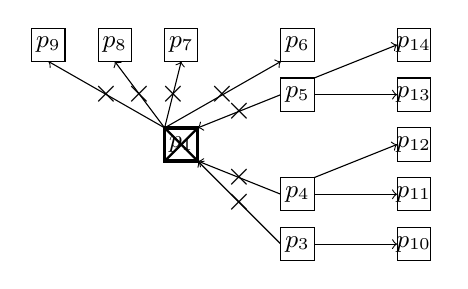
\begin{tikzpicture}[scale=1.2]

  \newcommand\X{35pt};
  \newcommand\Y{15pt};
  \large
  \draw[->](-5+\X, 1*\Y) --node{$\times$} ( 5pt,5pt);
  \draw[->](-5+\X, -1*\Y) --node{$\times$} ( 5pt,-5pt);
  \draw[->](-5+\X, -2*\Y) --node{$\times$} ( 5pt,-5pt);

  \draw[->](-5pt,5pt)--node{$\times$}(-10-2*\Y,-5+2*\Y); %% 1 -> 9
  \draw[->](-5pt,5pt)--node{$\times$}(-5-1*\Y,-5+2*\Y); %% 1 ->8 
  \draw[->](-5pt,5pt)--node{$\times$}(0pt,-5+2*\Y); %% 1 -> 7
  \draw[->](-5pt,5pt)--node{$\times$}(-5+\X,-5+2*\Y); %% 1 -> 6
  \normalsize
  \draw[->](5+ 1*\X, 5+ 1*\Y)--(-5+2*\X, 2*\Y); %% 5 -> 14
  \draw[->](5+1*\X,  1*\Y)--(-5+2*\X, 1*\Y); %% 5 -> 13 
  
  \draw[->](5+\X, 5-\Y) -- (-5+2*\X,0pt); %% 4 -> 12
  \draw[->](5+\X, -\Y) -- (-5+2*\X, -\Y); %% 4 -> 11
  
  \draw[->](5+\X, -2*\Y) -- (-5+2*\X, -2*\Y);
  
  \small
  \draw[fill=white,very thick]
  (0*\X, 0*\Y) node{$p_1$} +(-5pt,-5pt) rectangle +(5pt,5pt);
  \draw[thick] (-5pt,-5pt) -- (5pt,5pt);
  \draw[thick] (-5pt, 5pt) -- (5pt,-5pt);
  
  \draw[fill=white]
  (1*\X,1*\Y) node{$p_5$} +(-5pt,-5pt) rectangle +(5pt,5pt);
  \draw[fill=white]
  (1*\X,-1*\Y) node{$p_4$} +(-5pt,-5pt) rectangle +(5pt,5pt);
  \draw[fill=white]
  (1*\X,-2*\Y) node{$p_3$} +(-5pt,-5pt) rectangle +(5pt,5pt);

  \draw[fill=white](\X,2*\Y) node{$p_6$} +(-5pt,-5pt) rectangle +(5pt,5pt);

  \draw[fill=white]( 0*\X,2*\Y)
  node{$p_7$} +(-5pt,-5pt) rectangle +(5pt,5pt);
  \draw[fill=white](-5+-\Y,2*\Y)node{$p_8$} +(-5pt,-5pt) rectangle +(5pt,5pt);
  \draw[fill=white](-10+-2*\Y,2*\Y) node{$p_9$} +(-5pt,-5pt) rectangle +(5pt,5pt);
  
  \draw[fill=white](2*\X,2*\Y)node{$p_{14}$} +(-5pt,-5pt) rectangle +(5pt,5pt);
  \draw[fill=white](2*\X,1*\Y)node{$p_{13}$} +(-5pt,-5pt) rectangle +(5pt,5pt);
  \draw[fill=white](2*\X,0*\Y)node{$p_{12}$} +(-5pt,-5pt) rectangle +(5pt,5pt);
  \draw[fill=white](2*\X,-1*\Y)node{$p_{11}$}+(-5pt,-5pt) rectangle +(5pt,5pt);
  \draw[fill=white](2*\X,-2*\Y)node{$p_{10}$}+(-5pt,-5pt) rectangle +(5pt,5pt);

\end{tikzpicture}}
  \hspace{10pt}
  \subfloat[Figure B][The peer $p_3$, $p_4$, and $p_5$ notice that they
  cannot reach $p_1$ anymore.]{
    
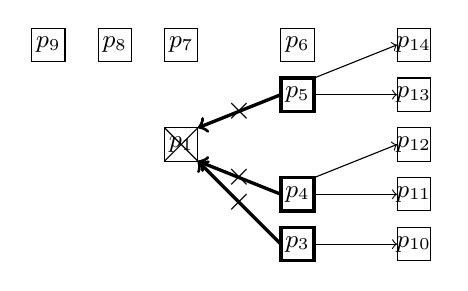
\begin{tikzpicture}[scale=1.2]

  \newcommand\X{35pt};
  \newcommand\Y{15pt};

  \large
  \draw[->, very thick](-5+\X, 1*\Y) -- node{$\times$} ( 5pt,5pt);
  \draw[->, very thick](-5+\X, -1*\Y) --node{$\times$} ( 5pt,-5pt);
  \draw[->, very thick](-5+\X, -2*\Y) --node{$\times$} ( 5pt,-5pt);

  \normalsize

  \draw[->](5+ 1*\X, 5+ 1*\Y)--(-5+2*\X, 2*\Y); %% 5 -> 14
  \draw[->](  5+1*\X, 1*\Y)--(-5+2*\X, 1*\Y); %% 5 -> 13 (v)
  
  \draw[->](5+\X, 5-\Y) -- (-5+2*\X,0pt); %% 4 -> 12
  \draw[->](5+\X, -\Y) -- (-5+2*\X, -\Y); %% 4 -> 11
  
  \draw[->](5+\X, -2*\Y) -- (-5+2*\X, -2*\Y);
  
  \small
  \draw[fill=white]
  (0*\X, 0*\Y) node{$p_1$} +(-5pt,-5pt) rectangle +(5pt,5pt);
  \draw (-5pt,-5pt) -- (5pt,5pt);
  \draw (-5pt, 5pt) -- (5pt,-5pt);
  
  \draw[fill=white, very thick]
  (1*\X,1*\Y) node{$p_5$} +(-5pt,-5pt) rectangle +(5pt,5pt);
  \draw[fill=white, very thick]
  (1*\X,-1*\Y) node{$p_4$} +(-5pt,-5pt) rectangle +(5pt,5pt);
  \draw[fill=white, very thick]
  (1*\X,-2*\Y) node{$p_3$} +(-5pt,-5pt) rectangle +(5pt,5pt);

  \draw[fill=white](\X,2*\Y) node{$p_6$} +(-5pt,-5pt) rectangle +(5pt,5pt);

  \draw[fill=white]( 0*\X,2*\Y)
  node{$p_7$} +(-5pt,-5pt) rectangle +(5pt,5pt);
  \draw[fill=white](-5+-\Y,2*\Y)node{$p_8$} +(-5pt,-5pt) rectangle +(5pt,5pt);
  \draw[fill=white](-10+-2*\Y,2*\Y) node{$p_9$} +(-5pt,-5pt) rectangle +(5pt,5pt);
  
  \draw[fill=white](2*\X,2*\Y)node{$p_{14}$} +(-5pt,-5pt) rectangle +(5pt,5pt);
  \draw[fill=white](2*\X,1*\Y)node{$p_{13}$} +(-5pt,-5pt) rectangle +(5pt,5pt);
  \draw[fill=white](2*\X,0*\Y)node{$p_{12}$} +(-5pt,-5pt) rectangle +(5pt,5pt);
  \draw[fill=white](2*\X,-1*\Y)node{$p_{11}$}+(-5pt,-5pt) rectangle +(5pt,5pt);
  \draw[fill=white](2*\X,-2*\Y)node{$p_{10}$}+(-5pt,-5pt) rectangle +(5pt,5pt);

\end{tikzpicture}}
  \hspace{10pt}
  \subfloat[Figure C][The peer $p_3$ and $p_5$ choose to establish
  a duplicate with one of their existing neighbor.]{
    
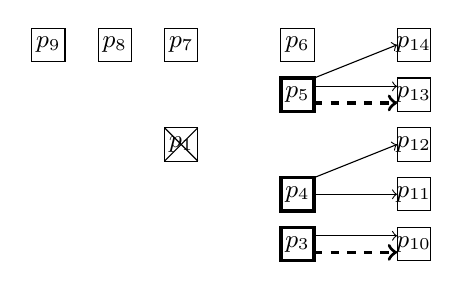
\begin{tikzpicture}[scale=1.2]

  \newcommand\X{35pt};
  \newcommand\Y{15pt};

  \draw[->](5+ 1*\X, 5+ 1*\Y)--(-5+2*\X, 2*\Y); %% 5 -> 14
  \draw[->](5+1*\X, 2.5+ 1*\Y)--(-5+2*\X, 2.5+ 1*\Y); %% 5 -> 13 (^)
  \draw[->,dashed, very thick]
  (  5+1*\X,-2.5+1*\Y)--(-5+2*\X,-2.5+1*\Y); %% 5 -> 13 (v)
  
  \draw[->](5+\X, 5-\Y) -- (-5+2*\X,0pt); %% 4 -> 12
  \draw[->](5+\X, -\Y) -- (-5+2*\X, -\Y); %% 4 -> 11
  
  \draw[->](5+\X, 2.5-2*\Y) -- (-5+2*\X, 2.5-2*\Y);
  \draw[->,dashed, very thick](5+\X, -2.5-2*\Y) -- (-5+2*\X , -2.5-2*\Y);
  
  \small
  \draw[fill=white]
  (0*\X, 0*\Y) node{$p_1$} +(-5pt,-5pt) rectangle +(5pt,5pt);
  \draw (-5pt,-5pt) -- (5pt,5pt);
  \draw (-5pt, 5pt) -- (5pt,-5pt);
  
  \draw[fill=white, very thick]
  (1*\X,1*\Y) node{$p_5$} +(-5pt,-5pt) rectangle +(5pt,5pt);
  \draw[fill=white, very thick]
  (1*\X,-1*\Y) node{$p_4$} +(-5pt,-5pt) rectangle +(5pt,5pt);
  \draw[fill=white, very thick]
  (1*\X,-2*\Y) node{$p_3$} +(-5pt,-5pt) rectangle +(5pt,5pt);

  \draw[fill=white](\X,2*\Y) node{$p_6$} +(-5pt,-5pt) rectangle +(5pt,5pt);

  \draw[fill=white]( 0*\X,2*\Y)
  node{$p_7$} +(-5pt,-5pt) rectangle +(5pt,5pt);
  \draw[fill=white](-5+-\Y,2*\Y)node{$p_8$} +(-5pt,-5pt) rectangle +(5pt,5pt);
  \draw[fill=white](-10+-2*\Y,2*\Y) node{$p_9$} +(-5pt,-5pt) rectangle +(5pt,5pt);
  
  \draw[fill=white](2*\X,2*\Y)node{$p_{14}$} +(-5pt,-5pt) rectangle +(5pt,5pt);
  \draw[fill=white](2*\X,1*\Y)node{$p_{13}$} +(-5pt,-5pt) rectangle +(5pt,5pt);
  \draw[fill=white](2*\X,0*\Y)node{$p_{12}$} +(-5pt,-5pt) rectangle +(5pt,5pt);
  \draw[fill=white](2*\X,-1*\Y)node{$p_{11}$}+(-5pt,-5pt) rectangle +(5pt,5pt);
  \draw[fill=white](2*\X,-2*\Y)node{$p_{10}$}+(-5pt,-5pt) rectangle +(5pt,5pt);

\end{tikzpicture}}
  \caption{\label{fig:crashexample}Example of \SCAMPLON{}'s crash/leaving
    handler. The scenario follows from prior examples after few other
    exchanges. Peer $p_1$ leaves the network without giving notice. With it,
    $7$ connections are down. Peers $p_3$, $p_4$, and $p_5$ have the
    crashed/left peer in their partial view. Peer $p_5$ has
    $1-{1\over{|\mathcal{P}_5|}}={2\over{3}}$ chance to replace the dead
    connections. In this case, it doubles the connection to
    $p_{13}$. Identically, $p_3$ and $p_4$ detect the crash/leaving and run the
    appropriate procedure. Only $p_3$ doubles one of its connection. In total,
    $5$ connections have been removed.}
\end{figure*}

Figure~\ref{fig:crashexample} depicts the \SCAMPLON{}'s crash/leaving
handler. The example shows that some peers reestablish connections if they
detect a dead connection. The probability depends on the partial view size of
each of these peer. In average, one of these peer will likely remove the
connection while the other peers will double one of their existing
connections. In this case, Peer $p_1$ injected $5$ connections when it
joined. It removes $7-2 =5 $ connections when it leaves. The global number of
connections remains logarithmic compared to the number of members in the
network. Nevertheless, we can see that connectedness is not entirely guaranteed
(only with the high probability implied by random graphs). Indeed, if Peer
$p_1$ is the sole bridge between two clusters, adding connections is not enough
to ensure connectedness (more details in Section~\ref{subsec:resilience}).

Note that extending the algorithms to handle three-way handshake is not
difficult: it only requires to keep track of the neighbor from where the
membership messages arrived, and forward the answer to this neighbor
accordingly. Also, there are few optimization concerning the establishments of
connections. For instance, when a peer $p$ starts an exchange with $q$, and $q$
has $p$ in its partial view, instead of inverting the link between $p$ and $q$,
and $q$ and $p$, \SCAMPLON{} does not change them. Another optimization
concerns a peer having a neighbor multiple times in its partial view. While
\SCAMPLON{} keeps such information in its partial view, only one connection per
neighbor is truly necessary.

To summarize, \SCAMPLON{} provides:
\begin{inparaenum}[(i)]
\item a logarithmically increasing partial view size compared to the global
  network size,
\item a constant complexity to establish the connections,
\item an exponentially fast convergence to a random graph.
\end{inparaenum}
Providing these three properties, \SCAMPLON{} improves the state-of-the-art
approaches~\cite{ganesh2001scamp,voulgaris2005cyclon} in the traditional
connection set-up. Furthermore, the improvement becomes crucial in the context
of three-way handshake connection set-up.  The latter becomes increasingly
important with the appearance of technologies allowing peer-to-peer within
modern web browsers.  The next section aims to demonstrate experimentally the
behavior of \SCAMPLON{}. In particular, it aims to highlight the aforementioned
properties.


%%% Local Variables:
%%% mode: latex
%%% TeX-master: "../paper"
%%% End:

\section{Experimentation}
\label{sec:experiments}

In this section we examine the properties of \SCAMPLON{} and compare them to
properties of \CYCLON{}, a state-of-the-art cyclic peer sampling service.  As
\CYCLON{} uses fixed-sized partial views, we must predefine its partial view
size $c$.  As shown by Erd{\H o}s and R{\' e}nyi\cite{erdos1959random} random
graphs with less than $(|\mathcal{N}|*\ln|\mathcal{N}|)$ connections are likely
to partition - which is not desired for random peer sampling services.  We want
\CYCLON{} to be optimal for a network size of 1000 peers so we set the partial
view size to $c=7\approx \ln{1000}$ while in each cycle we exchange $l=3$
peers.  We call \CYCLON{} undersized when $\ln{|\mathcal{N}}| > c$, oversized
when $\ln{|\mathcal{N}|} < c$ and optimal when $\ln{|\mathcal{N}|} \approx c$.
The experiments\footnote{Implementation:
  https://github.com/anonymous/anonymous4now} involve up to 500,000 nodes and
are carried out on \PEERSIM{} \cite{peersim}, a simulator for peer-to-peer
networks.  We define a cycle as $\Delta t$ in which each peer has executed its
active protocol once.

We inspect three properties characteristic for random graphs, the \emph{average
  clustering coefficient}~\ref{subsec:cluster}, the \emph{average shortest path
  length}~\ref{subsec:avg} and \emph{the partial view size
  distribution}~\ref{subsec:dist}. Additionally, we investigate on
\emph{robustness to random failures}.

\subsection{Clustering coefficient}
\label{subsec:cluster}

\begin{figure}
  \centering
  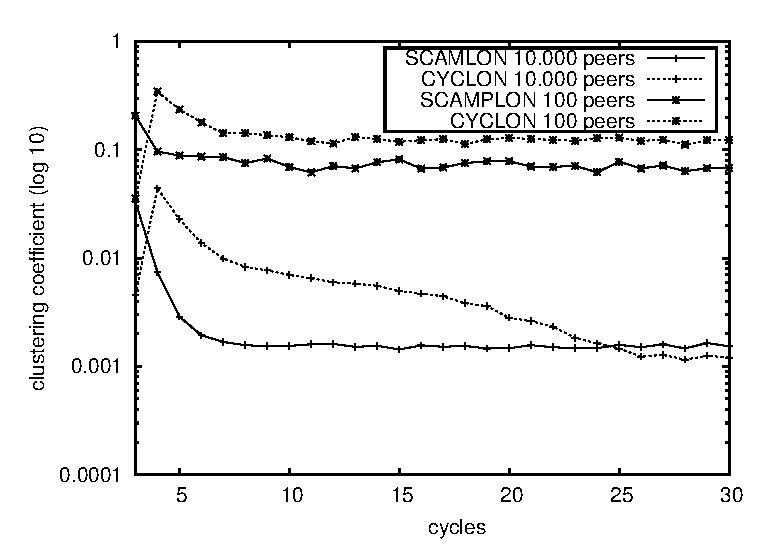
\includegraphics[width=0.49\textwidth]{img/cluster.eps}
  \caption{\label{fig:clustering}Clustering coefficient}
\end{figure}

\begin{asparadesc}
\item[Objective:] We want to evaluate to what degree \SCAMPLON{} generates
  clusters in the overlay.  To satisfy the random peer sampling objective it is
  desired that the network has few clusters, thus has a sufficiently low
  clustering coefficient.  This is important for various reasons: first: highly
  clustered networks show poor load-balancing when messages are broadcast as
  peers have a high chance of receiving a message multiple times through their
  neighbors; and second: A network consisting of poorly connected clusters is
  less robust regarding peers failing or simply leaving the overlay to
  disconnect the graph.
\item[Description:] The average clustering coefficient $\overline{C}$ measures
  the connectivity of each peer's neighborhood in the network.
  \begin{equation}
    \overline{C} = {1\over |\mathcal{N}|}\sum\limits_{x\in\mathcal{N}}C_x
  \end{equation}
  where $C_x$ is the local clustering coefficient of Peer $p_x$. The higher the
  coefficient, the more likely the network contains cliques.  The experiments
  involve 100, 1000, 10000 and 100000 peers.
\item[Results:] Figure \ref{fig:clustering} shows that \SCAMPLON{} converges
  faster than \CYCLON{}.  Furthermore, oversized \CYCLON{} converges to a
  higher value than \SCAMPLON while it converges to a lower one when
  undersized.
\item[Reasons:] The experiments yield the expected results: \SCAMPLON{}
  converges faster as it is not constraint by a fixed, artificial barrier
  $l$.  On the other hand, \CYCLON{} yields a lower clustering coefficient on
  convergence when undersized.  This can be explained by the fact that peers in
  an undersized \CYCLON{} overlay have less connections and thus have a lower
  probability of forming cliques.  This, however, makes it more vulnerable to
  node failure and churn.
\end{asparadesc}

\subsection{Average path length}
\label{subsec:avg}
\begin{figure}
  \centering
  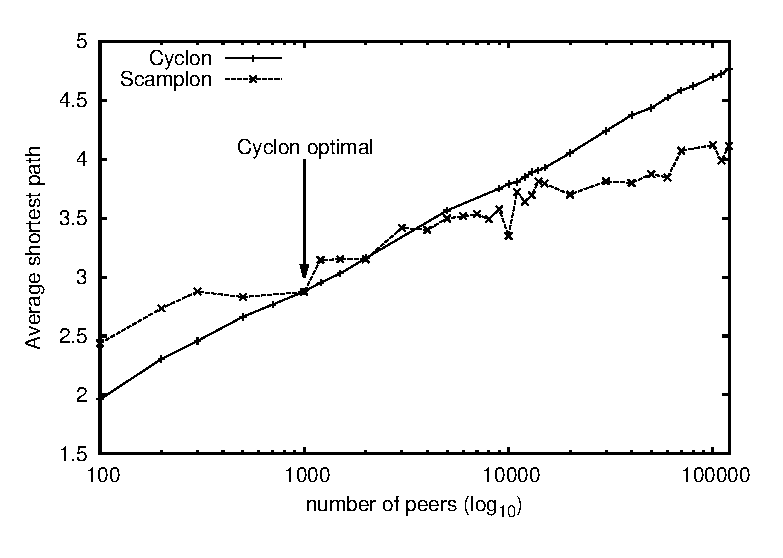
\includegraphics[width=0.49\textwidth]{img/avgpath.eps}
  \caption{\label{fig:avgpath}Average shortest path}
\end{figure}

\begin{asparadesc}
\item[Objective:] In this experiment we examine the shortest path length that
  peers have to all other nodes in the network.  Messages should disseminate
  quickly into the network which makes it crucial that the shortest path to
  other peers is, in fact, short.
\item[Description:] The average path length is the average of the shortest path
  length between peers in the graph. It counts the minimum number of hops to
  reach a peer from another given peer.  For performance reasons, we select a
  subset of 7 nodes, calculate their average shortest path and average it by 7.
\item[Results:] Figure~\ref{fig:avgpath} shows that \CYCLON{}, when oversized,
  yield a shorter average path length then \SCAMPLON{} but is quickly exceeded
  when undersized.
  %after its optimal partial view size is exceeded \SCAMPLON{} yields a shorter
  %path.
\item[Reasons:] While oversized \CYCLON{} is much better connected into the
  graph and thus yields a lower average path length then \SCAMPLON{}, as soon
  as it is undersized, \SCAMPLON{} is, thanks to bigger partial views, better
  connected into the graph and, consequently, yields the shorter average path
  length.
\end{asparadesc}

\subsection{Partial view size distribution}
\label{subsec:dist}

\begin{figure}
  \centering
  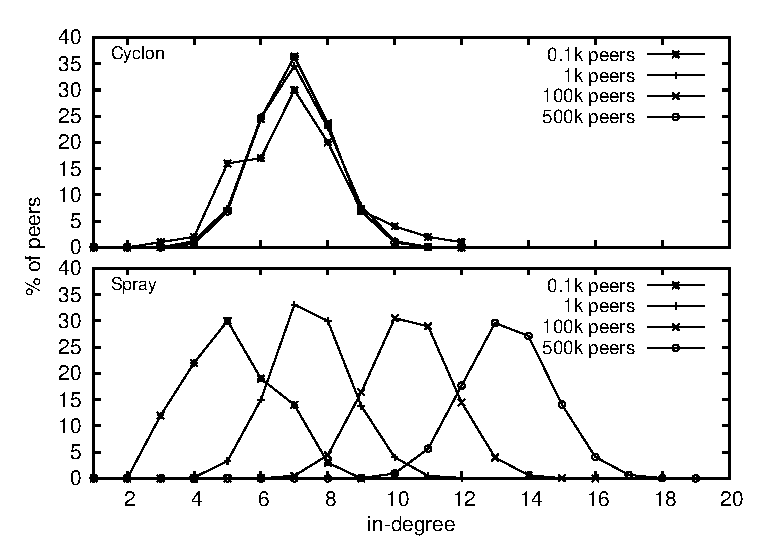
\includegraphics[width=0.49\textwidth]{img/histo.eps}
  \caption{\label{fig:histo}In-degree distribution}
\end{figure}

\begin{asparadesc}
\item[Objective:] As the degree distribution shows the existence of both,
  weakly connected peers as well as strongly connected hubs, it helps to
  analyze the robustness of the overlay when failure is present.  Additionally,
  it indicates how well-distributed links in the network are which
  helps to approximate the resource usage across peers.
\item[Description:] As the overlay can be represented as a directed graph we
  distinguish between out-degree which determines to how many other nodes a
  peer points, and the in-degree which determines from how many other peers a
  certain peer is referenced.  We concentrate on the in-degree for better
  comparison as in \CYCLON{} the out-degree is fixed ($c$).
\item[Results:] Figure~\ref{fig:histo} shows the in-degree distribution of
  \CYCLON{} and \SCAMPLON{}.  In \CYCLON{} the number of peers in the overlay
  has no influence on the degree distribution always as it always gathers
  around the selected partial view size $c$.  In \SCAMPLON{}, however, the
  degree distribution depends logarithmically on the network size and grows and
  shrinks with the network.
\item[Reasons:] \CYCLON{}'s fixed partial view size accounts for its rigid
  behavior.  In \SCAMPLON{} the distribution is much more fluid...
\end{asparadesc}

\subsection{Dynamic network}

\begin{figure}
  \centering
  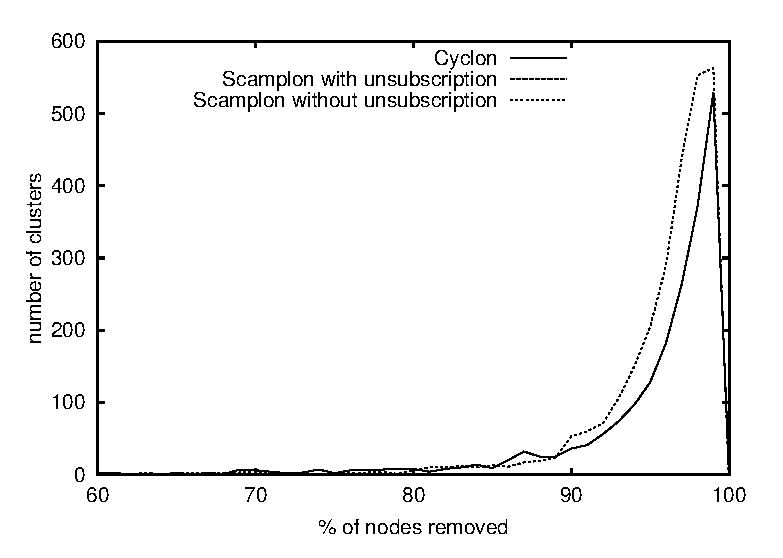
\includegraphics[width=0.49\textwidth]{img/churn.eps}
  \caption{\label{fig:churn}Churn effect}
\end{figure}

\begin{asparadesc}
\item[Objective:] To highlight that \SCAMPLON{} is adaptive, i.e., the total
  number of connections reflects the network membership. Furthermore, the
  connections are quickly spread among the members.
\item[Description:] The first half of the experimentation, $2,500$ peers are
  added $4$ times successively by intervals of $10$ cycles each. Thus, the
  network size goes from $0$ to $10,000$ peers in $40$ rounds. Then, half of
  the network leaves without giving notice ($5,000$ peers). Finally, $2,500$
  peers join two additional times. The final network size is $10,000$
  members. The measurements concern
  \begin{inparaenum}
  \item the number of connections in the network over cycles,
  \item the variance of the partial view sizes over cycles
    (cf. Section~\ref{subsec:cyclic}).
  \end{inparaenum}
\item[Results:] Figure~\ref{fig:churn} shows the result of the experiment. The
  x-axis represents the cycles (i.e. the arbitrary unit time frame). The top
  figure shows the number of connections established in the network (scale
  $\times 10^3$). The bottom figure shows the variance in the partial view size
  of the members. We can see that at each batch of joinings, the connection
  number grows to reflect the needs of the new network membership. The
  observation is consistent with the variance measures. Indeed, at each batch
  of insertions, the variance suddenly grows. Then, it exponentially decreases
  and converges to zero in less than $10$ cycles. The variance is higher when
  the network size is lower. For instance, the first $2,500$ peers lead to the
  highest variance. At the $40^{th}$ rounds, half of the peers
  leave/crash. Around half of the connections are directly removed without
  disturbing the variance of partial views. The $10$ following cycles show a
  slight decrease of connections. Then new members are introduced in the
  network yielding the same results as earlier joinings.
\item[Reasons:] Since the partial views of \SCAMPLON{} adapt themselves to the
  network size, the number of connections grows as the network membership
  grows.  The peaks in variance correspond to the joining parts of the
  experiment. The disparity comes from the fact that new peers arrive in the
  network with a small partial view. The peaks are smaller when the network is
  larger. Indeed, the peers - which already were network members before the new
  arrivals - had a few rounds to exchanges and even up their partial views. As
  consequence, it lessens the weight of joinings. The removal of $5,000$ peers
  do not disturb the variance since they are made at random. Thus, no peers
  suffer more of these removals than others. The slightly decreasing number of
  connections after the removal is due to peers realizing that some connections
  are dead, leading to a probabilistic removal
  (cf. Algorithm~\ref{algo:unreachable}).
\end{asparadesc}

\subsection{Massive failures}
\label{subsec:resilience}

\begin{figure}
  \centering
  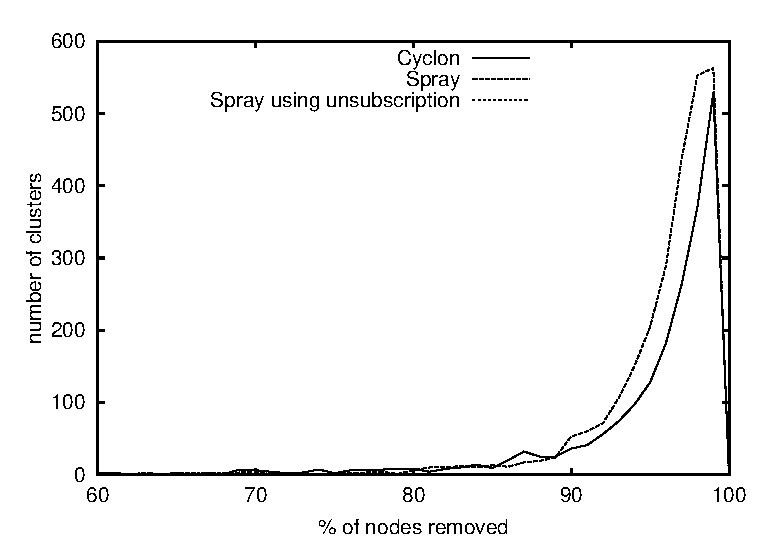
\includegraphics[width=0.49\textwidth]{img/resilience.eps}
  \caption{\label{fig:resilience}Resilience to massive failure}
\end{figure}


\begin{algorithm}

\small
\algrenewcommand{\algorithmiccomment}[1]{\hskip2em$\rhd$ #1}

\newcommand{\comment}[1]{$\rhd$ #1}

\algblockdefx[initially]{initially}{endInitially}
  [0] {\textbf{INITIALLY:}}

\algblockdefx[pas]{pas}{endPas}
  [0] {\textbf{EVENTS:}}

\newcommand{\LINEFOR}[2]{%
  \algorithmicfor\ {#1}\ \algorithmicdo\ {#2} %
  }

\newcommand{\LINEIFTHEN}[2]{%
  \algorithmicif\ {#1}\ \algorithmicthen\ {#2} %
  }

\newcommand{\INDSTATE}[1][1]{\State\hspace{\algorithmicindent}}

\begin{algorithmic}[1]
  \Statex
  \initially
  \State $\mathcal{I}$ \hfill \label{line:inview}
  \comment{set of peers targeting us ($p$) in their partial view}
  \endInitially

  \pas
    \Function{unSubscribe}{\ }
    \For{$i\leftarrow 0$ \textbf{to} $min(|\mathcal{P}|,\, |\mathcal{P}|-1)$ 
      \label{line:bridge}}    
    \State \textbf{let} $\langle n,\,\_ \,\rangle \leftarrow \mathcal{P}[i]$;
    \State $sendTo(\, \mathcal{I}[\,i\%|\mathcal{I}|\,],\, 'unSubs',\, n)$;
    \EndFor
    \EndFunction
    \Statex
    \Function{onUnSubs}{$o, \, n$} 
    \hfill \comment{$o$: origin; $n$: neighbor to add}
    \State $\mathcal{P}\leftarrow (\mathcal{P}\setminus o)
    \uplus\{\langle n,\,0\rangle\}$;
    \EndFunction
  \endPas
\end{algorithmic}

\caption{\label{algo:unsubscription}Unsubscription protocol from
  \SCAMP{}~\cite{ganesh2003peer}}
\end{algorithm}

\begin{asparadesc}
\item[Objective:] 
\item[Description:] Algorithm~\ref{algo:unsubscription} shows the
  unsubscription protocol which guarantees connectedness (WITH HIGH PROBA?)
  upon the assumption that an \emph{in view} $\mathcal{I}$ is maintained
  (cf. Line~\ref{line:inview}) along with bidirectional connections. The set of
  peers which have a particular peer in their partial view populate the
  latter's in view. When a peer leaves, it actively contributes to repair the
  network by acting like a bridge between its in view $\mathcal{I}$ and its
  partial view $\mathcal{P}$. As consequence, the neighbors from $\mathcal{I}$
  add each peer from the leaving peer's partial view in their own partial view.
  Except for one peer (cf. Line~\ref{line:bridge}), it guarantees that these
  peers stay connected, i.e., that at least one partial view references them.

\item[Results:]
\item[Reasons:]
\end{asparadesc}

\subsection{Degeneration}

\begin{figure}
  \centering 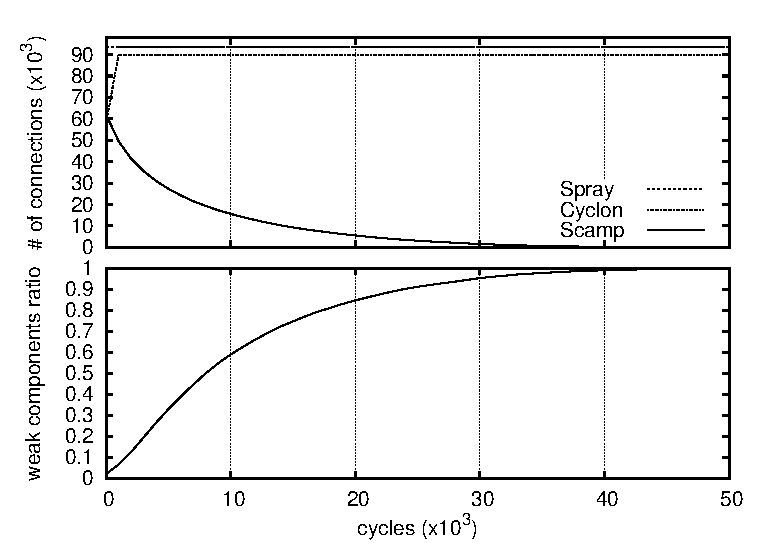
\includegraphics[width=0.49\textwidth]{img/degen.eps}
  \caption{\label{fig:degen}Degeneration of static network} \end{figure}

\begin{asparadesc} \item[Objective:] \SCAMPLON{}, especially when using
        \emph{handshaking}, is vulnerable to message loss. When messages can
        be lost, a static \SCAMPLON{} overlay where peers neither join
        nor leave will slowly degenerate.
        The reason for this can be found in Algorithm~\ref{algo:unreachable} 
        where arcs are potentially lost when a message is lost.
        As static protocols like \CYCLON{} are not prone to this degeneration
        we compare with another adaptive probabilistic protocol,
        \SCAMP{}, instead. We adapted \SCAMP{} so that its lease-mechanism preserves
        the total number of arcs in the network.
        This experiment focuses on two features: the total number of arcs in the 
        graph and the number of weak components.
\item[Description:]
    As previously shown, the number of arcs in the network should be
    $|\mathcal{N}|\log{|\mathcal{N}|}$ for the overlay to be robust. A weak
    component $\mathcal{W}$ of a graph $G$ is a maximum subgraph where the direction
    is ignored.
    Naturally, we want the number of weak components $|\mathcal{W}|$ to be $1$,
    meaning that the whole network is connected.
    When the overlay consists of more than one component, the network is disconnected.
    Unlike with strong component where the direction is taken into account, \SCAMPLON{}
    cannot repair itself when more than one weak component is present.
    The experiment involves handshaking and is conducted with an overlay consisting
    of $10,000$ peers over a period of $100,000$ cycles and a probability of
    $\frac{1}{1000}$ that a link fails. \TODO{BRICE: PLEASE ELABORATE YOUR CALCS}

\item[Results:]
    The x-axis in Figure~\ref{fig:degen} shows the number of cycles the protocol was
    executed.
    The upper graphs y-axis represents the total number of arcs in the
    overlay while the lower graphs y-axis shows the percentage that weak components
    make up of the total network: $\frac{|\mathcal{W}|}{|\mathcal{N}|}$.
    We clearly see that \SCAMPLON{} degenerates much slower than \SCAMP{} and that
    it becomes disconnected very late while \SCAMP{} collapses quickly.

\item[Reasons:]
    As \SCAMP{} must maintain much more links than \SCAMPLON{} when establising a
    connection it has a higher probability of losing arcs which, in turn, let it
    degenerate much quicker.
    Furthermore, while in \SCAMPLON{} we can easily predict if a link failed or if
    the node failed and thus we can stop the degeneration this is not possible in
    \SCAMP{} as it cannot be easiliy predicted for when a link failed due to its
    random walk nature.

\end{asparadesc}

%% \subsection{Synthesis}

%%% Local Variables:
%%% mode: latex
%%% TeX-master: "../paper"
%%% End:


\section{Conclusion and perspectives}
\label{sec:conclusion}

%%\TODO{A lot to change. Includes perspective with security, maybe problems of
%%  merging etc.}

% WebRTC opened a new playground for large-scale distributed
% applications deployed on a network of browsers. Browsers as an
% infrastructure ease the deployment of large-scale distributed
% applications for end-users. Yet, WebRTC exacerbates the limitations,
% in term of adaptiveness and reliability, of a core component of many
% large-scale distributed applications: peer-sampling protocols.

In this paper, we described \SPRAY, an adaptive-by-design random peer sampling
approach designed to fit WebRTC's constraints.  \SPRAY provides:
\begin{inparaenum}[(i)]
\item logarithmically growing partial views reflecting the global network size,
\item constant time complexity on connection establishments using solely
  neighbor-to-neighbor interactions.
% \item an exponentially fast convergence to an overlay network exposing
%   properties similar to random graphs.
\end{inparaenum}
Our experiments demonstrate how \SPRAY's adaptiveness improves the performance
of random peer sampling when the size of the network changes. In particular, the
average shortest path length scales better, the in-degree evolves with the
network size, and it converges faster.  Adaptiveness comes at the price of
duplicates in the partial views. However, our simulations supported by
theoretical analysis show that the number of duplicates remains very low and
becomes negligible in large networks.

To highlight the improvement brought by such protocol, we demonstrated
how a broadcast protocol can take advantage of adaptiveness of \SPRAY to
adjust the fanout and handle sudden burst of popularity. We also built
\CRATE, a decentralized collaborative editor directly accessible in
web browsers with a full implementation of \SPRAY on top of WebRTC. We
launched experiments involving up to 600 browsers showing that message
dissemination highly benefits from adaptive neighborhoods.

\SPRAY makes building scalable decentralized applications in browsers
easy and accessible.  Developers do not require to oversee the network
size targeted by their applications. Just the same as for broadcast,
many topology optimization protocols (e.g. about geolocalization,
latency, or preferences) rely on random peer sampling protocol such as
the generic algorithms T-Man~\cite{jelasity2009tman} and
Vicinity~\cite{voulgaris2005epidemic}. \SPRAY allows such protocols to
take benefict from its self-adjusting partial views.

% Future work includes investigations on topology managers such as
% T-Man~\cite{jelasity2009tman} or
% Vicinity~\cite{voulgaris2005epidemic}. Indeed, they traditionally rely
% on random peer sampling approaches using fixed-size partial
% view. Thus, they maintain a fixed-size view of their most closely
% related neighbors using a ranking function. With \SPRAY, we could
% extend their behavior to use dynamic partial views.

%%% Local Variables:
%%% mode: latex
%%% TeX-master: "../paper"
%%% End:

%
\section*{Acknowledgment}

This work was partially funded by the French ANR project SocioPlug
(ANR-13-INFR-0003), and by the DeSceNt project granted by the Labex CominLabs
excellence laboratory (ANR-10-LABX-07-01).

%%% Local Variables:
%%% mode: latex
%%% TeX-master: "../paper"
%%% End:


%% Bibliographie
\bibliographystyle{abbrv}
\bibliography{bibliographie}
\clearpage
  
\end{document}

%%% Local Variables:
%%% mode: latex
%%% TeX-master: t
%%% End:
